\documentclass[11pt,a4paper]{article}
\usepackage[margin=2cm]{geometry}
\usepackage{lmodern}
\usepackage[T1]{fontenc}
\usepackage{amsmath,amssymb}
\usepackage{booktabs,array,tabularx,xltabular}
\usepackage{enumitem}
\usepackage{xcolor}
\usepackage[most]{tcolorbox}
\usepackage{titlesec}
\usepackage{graphicx}
\usepackage{float}
\usepackage[font=small,labelfont={bf,color=headblue},skip=4pt]{caption}
\usepackage[colorlinks=true,linkcolor=headblue,urlcolor=blue!50!black]{hyperref}

\definecolor{headblue}{RGB}{38,70,120}
\titleformat{\section}{\Large\bfseries\color{headblue}}{\thesection}{0.8em}{}[{\color{black}\titlerule}]
\titleformat{\subsection}{\large\bfseries\color{headblue}}{\thesubsection}{0.8em}{}
\titleformat{\subsubsection}{\normalsize\bfseries\color{headblue}}{\thesubsubsection}{0.8em}{}
\titlespacing*{\section}{0pt}{12pt}{6pt}
\titlespacing*{\subsection}{0pt}{9pt}{3pt}
\titlespacing*{\subsubsection}{0pt}{7pt}{2pt}
\setlength{\parindent}{0pt}
\setlength{\parskip}{5pt}
\setlist{itemsep=2pt,topsep=2pt}
\setlength{\emergencystretch}{3em}
\renewcommand{\arraystretch}{1.12}
\setlength{\tabcolsep}{4.5pt}
\setlength{\LTpre}{2pt}\setlength{\LTpost}{2pt}
\allowdisplaybreaks
\newtcolorbox{keybox}{colback=blue!3,colframe=headblue!60,boxrule=0.5pt,arc=2mm,left=2mm,right=2mm,top=1mm,bottom=1mm}
\newtcolorbox{insum}{colback=green!3,colframe=green!40!black,boxrule=0.4pt,arc=1.5mm,left=2mm,right=2mm,top=0.5mm,bottom=0.5mm,fontupper=\small}
\newcommand{\inshort}[1]{\begin{insum}\textbf{In short.} #1\end{insum}}
\newcommand{\pct}{\,\%}

% generated by make_figures.py
\newcommand{\NInst}{560}
\newcommand{\NOpt}{256}
\newcommand{\NTL}{223}
\newcommand{\NNone}{30}
\newcommand{\NInf}{51}
\newcommand{\NValid}{479}
\newcommand{\GapMed}{4.2}
\newcommand{\GapMax}{26.9}
\newcommand{\NEV}{24250}
\newcommand{\NFree}{20584}
\newcommand{\NStranded}{3666}
\newcommand{\TimeLimit}{300}
\newcommand{\Workers}{8}
\newcommand{\Threads}{4}
\newcommand{\InfSame}{the same}
\newcommand{\VanAll}{7.0}
\newcommand{\VanLowOpt}{0.0}
\newcommand{\VanSixSeven}{7.7}
\newcommand{\VanSevenEight}{16.6}
\newcommand{\VanEightNine}{35.5}
\newcommand{\VanNineTen}{31.4}
\newcommand{\VanTopAll}{31.7}
\newcommand{\VanBotAll}{0.9}
\newcommand{\LowVanOpt}{0}
\newcommand{\LowVanTL}{74}
\newcommand{\ThetaVan}{0.74}
\newcommand{\ThetaFCS}{0.48}
\newcommand{\PressLow}{0.14}
\newcommand{\PressHigh}{0.41}
\newcommand{\QLow}{0.03}
\newcommand{\QueuingLow}{0.4}
\newcommand{\TopLow}{43.3}
\newcommand{\LowQLow}{0.05}
\newcommand{\TopQLow}{0.00}
\newcommand{\QMid}{0.08}
\newcommand{\QueuingMid}{1.3}
\newcommand{\TopMid}{27.8}
\newcommand{\LowQMid}{0.13}
\newcommand{\TopQMid}{0.00}
\newcommand{\QHigh}{4.08}
\newcommand{\QueuingHigh}{20.9}
\newcommand{\TopHigh}{21.1}
\newcommand{\LowQHigh}{8.38}
\newcommand{\TopQHigh}{0.62}
\newcommand{\QShareBottom}{72.8}
\newcommand{\UShareBottom}{35.6}
\newcommand{\QShareTop}{1.1}
\newcommand{\UShareTop}{7.2}
\newcommand{\DriveBot}{2.69}
\newcommand{\DriveTop}{1.78}
\newcommand{\TopShort}{27.3}
\newcommand{\PressShort}{0.53}
\newcommand{\TopLong}{35.8}
\newcommand{\PressLong}{0.45}
\newcommand{\PaidBot}{302}
\newcommand{\PaidTop}{369}
\newcommand{\FeltBot}{585}
\newcommand{\FeltTop}{694}
\newcommand{\MoneyBot}{410}
\newcommand{\MoneyTop}{230}
\newcommand{\TimeBot}{175}
\newcommand{\TimeTop}{464}
\newcommand{\ZOne}{0.8}
\newcommand{\ZTwo}{2.3}
\newcommand{\ZThree}{6.9}
\newcommand{\ZFour}{19.6}
\newcommand{\ZFive}{35.3}
\newcommand{\ZSix}{35.1}
\newcommand{\ZOperator}{28.8}
\newcommand{\ZCustomer}{71.2}
\newcommand{\VanWaitBot}{142}
\newcommand{\VanWaitTop}{9}
\newcommand{\AME}{4.0}
\newcommand{\AMEHigh}{2.5}
\newcommand{\AMENotHigh}{4.8}
\newcommand{\LogitAcc}{93.1}
\newcommand{\LogitN}{20584}

% generated by make_comprehensive.py
\newcommand{\NValidC}{479}
\newcommand{\NEVC}{24250}
\newcommand{\NFreeC}{20584}
\newcommand{\ZperMean}{938}
\newcommand{\ZperMin}{812}
\newcommand{\ZperMax}{1233}
\newcommand{\NQueued}{1414}
\newcommand{\NFCSfree}{19147}
\newcommand{\CorrThetaVan}{0.30}
\newcommand{\CorrThetaQueue}{-0.17}
\newcommand{\CorrPressQueue}{0.35}
\newcommand{\CorrThetaTime}{-0.13}
\newcommand{\CorrEPay}{0.89}
\newcommand{\CorrNearVan}{0.09}
\newcommand{\ElOperator}{28.8}
\newcommand{\ElMoney}{36.2}
\newcommand{\ElTariffs}{36.2}
\newcommand{\ElTime}{35.1}
\newcommand{\ElPiF}{14.6}
\newcommand{\ElCF}{6.9}
\newcommand{\ElPF}{25.7}
\newcommand{\ElPM}{9.7}
\newcommand{\ElMuZero}{26.9}
\newcommand{\ElMuOne}{9.3}
\newcommand{\ElCCOne}{22.0}
\newcommand{\ElCCZero}{2.4}
\newcommand{\ElCQOne}{0.86}
\newcommand{\ElCQZero}{0.20}
\newcommand{\ElCVOne}{3.8}
\newcommand{\ElCDOne}{4.9}
\newcommand{\GunRows}{10903}
\newcommand{\GunBind}{13.0}
\newcommand{\GunMean}{11.6}
\newcommand{\GunMed}{10.4}
\newcommand{\GunMax}{44.2}
\newcommand{\VanBind}{40.6}
\newcommand{\VanMean}{4.5}
\newcommand{\ArrMean}{11.5}
\newcommand{\RelMean}{3.8}
\newcommand{\PatRows}{19147}
\newcommand{\DeadRows}{25289}
\newcommand{\GunBindHigh}{60.3}
\newcommand{\GunBindLow}{0.5}
\newcommand{\GunOccBot}{7.2}
\newcommand{\GunOccTop}{18.5}
\newcommand{\GunFolBot}{21.8}
\newcommand{\GunFolTop}{6.0}
\newcommand{\PassedBot}{-5.08}
\newcommand{\PassedTop}{-20.85}
\newcommand{\DPFmean}{598}
\newcommand{\DPFmed}{546}
\newcommand{\DPFmax}{2567}
\newcommand{\DPMmean}{60}
\newcommand{\DPMmax}{274}
\newcommand{\DPFcong}{12.3}
\newcommand{\DPFperEV}{11.2}
\newcommand{\DTnonzero}{0}
\newcommand{\ThetaStar}{0.66}
\newcommand{\DeltaZero}{371}
\newcommand{\DeltaOne}{-191}
\newcommand{\ThetaStarDispatch}{3.33}
\newcommand{\ThetaStarQueue}{0.44}
\newcommand{\ThetaStarWait}{0.90}
\newcommand{\ThetaStarSmallE}{0.67}
\newcommand{\ThetaStarBigE}{0.65}
\newcommand{\ThetaStarFar}{0.48}
\newcommand{\ThetaStarNear}{0.79}
\newcommand{\DeltaDispatchOne}{1309}
\newcommand{\KappaTypical}{124}
\newcommand{\VansN}{1039}
\newcommand{\VansFull}{54.5}
\newcommand{\VanSeatsStranded}{71.8}
\newcommand{\VansBatt}{28.4}
\newcommand{\VansTime}{20.4}
\newcommand{\TightSeats}{61.2}
\newcommand{\TightBatt}{8.5}
\newcommand{\TightTime}{30.3}
\newcommand{\PerRsBot}{1.94}
\newcommand{\PerRsTop}{1.88}
\newcommand{\PerKWhBot}{15.7}
\newcommand{\PerKWhTop}{18.4}
\newcommand{\TimeShareBot}{29.9}
\newcommand{\TimeShareTop}{66.9}
\newcommand{\GreedyCost}{463}
\newcommand{\GreedyFinish}{11}
\newcommand{\GreedyNone}{86}
\newcommand{\BinHundred}{56,222}
\newcommand{\ConHundred}{171,924}
\newcommand{\InfProven}{51}
\newcommand{\InfTotal}{51}
\newcommand{\LateExample}{EV-RC105\_n10: EV 4 requests at minute 151, needs at least 92 min to charge, $T=240$}
\newcommand{\UnsolvedPress}{1.31}
\newcommand{\SolvedPressSame}{1.06}
\newcommand{\AllPressMean}{0.39}


\begin{document}

\begin{center}
{\LARGE\bfseries\color{headblue} EV Charging Network Optimisation\\[2pt] with Income-Based Market Segmentation}\\[8pt]
{\large Comprehensive results report: assumptions, exploratory analysis, shadow prices and sensitivity}\\[6pt]
{\normalsize CP 320 Operations Research for Mobility, course project}\\[2pt]
{\normalsize Yakshith Maddineni (SR 26080) \quad\textperiodcentered\quad Kartikeya Gaur (SR 26371)}\\[2pt]
{\normalsize 22 November 2026}
\end{center}

\begin{keybox}
{\color{headblue}\textbf{How to read this report}}\\
The report has three parts. \textbf{Part I} lists every assumption behind the model, the data and the run, with the reason for each and what changes if it is relaxed. \textbf{Part II} is a basic exploratory analysis of the \NInst{} solved instances. \textbf{Part III} analyses the results point by point: the anatomy of the objective function, the shadow prices (dual values) of the plans, the income threshold predicted by theory, the choice of resource, queues, peak demand, horizons, the vans, equity, computation, infeasibility and sensitivity to the income distribution. Every subsection ends with a green \emph{In short} box. Section~\ref{sec:glossary} explains every technical term; a term in \emph{italics} on first use is in the glossary.
\end{keybox}

\begin{keybox}
{\color{headblue}\textbf{The main results in ten lines}}
\begin{enumerate}[leftmargin=1.4em,itemsep=1pt]
  \item All \NValid{} plans are valid; the \NInf{} infeasible instances are infeasible because of the data (Section~\ref{sec:infeasible}).
  \item In proven-optimal plans no customer with $\theta<0.4$ gets a van; the van share rises to \VanEightNine\pct{} at $\theta$ 0.8--0.9 (Section~\ref{sec:choice}).
  \item Theory predicts an income threshold $\theta^{*}=\ThetaStar$ for a typical EV; the data show the step at the same place (Section~\ref{sec:threshold}).
  \item A van is never sent out for a free-choice EV alone: its dispatch cost pushes $\theta^{*}$ to \ThetaStarDispatch{}. Vans leave for the stranded EVs and the rich fill the seats left over (Sections~\ref{sec:threshold}, \ref{sec:vans}).
  \item The poorest 40\pct{} of station users do \QShareBottom\pct{} of all queueing; the richest 20\pct{} do \QShareTop\pct{} (Section~\ref{sec:queues}).
  \item Shadow prices show the congestion: a gun-minute is worth \GunMean{} Rs on average when it is scarce, almost always because a richer EV holds the gun while a poorer one waits (Section~\ref{sec:duals}).
  \item Patience limits and the deadline $T$ have zero shadow price in every plan; they matter only through which plans are possible (Section~\ref{sec:duals}).
  \item One more kW of station-gun power is worth about \DPFmean{} Rs per instance (Section~\ref{sec:duals}).
  \item The objective is most sensitive to the FCS tariff, the money sensitivity of low incomes, the value of FCS charging time of high incomes and the grid price (Section~\ref{sec:anatomy}).
  \item In short-horizon families the vans run out of \emph{time}; in long-horizon families they run out of \emph{seats} (Section~\ref{sec:vans}).
\end{enumerate}
\end{keybox}

\tableofcontents
\newpage

%=====================================================================
\section{Glossary}
\label{sec:glossary}

\begin{xltabular}{\textwidth}{@{}>{\raggedright\arraybackslash}p{4.0cm}X@{}}
\toprule
\textbf{Term} & \textbf{Meaning} \\
\midrule
\endhead
EV & Electric vehicle that asks to be charged during the planning period. \\
FCS, gun & Fixed charging station; each has 2 \emph{guns} (charging points) of 22\,kW. A gun charges one EV at a time. \\
MCS, van & Mobile charging station: a van with a 150\,kWh battery that drives to parked EVs and charges them one at a time at 30\,kW, starting and ending at the depot. \\
Request time $r_i$ & Minute at which EV $i$ asks for charging. \\
Horizon $T$ & Length of the planning period in minutes; every EV must be fully charged and every van back by $T$. \\
Stranded EV & EV whose remaining range is shorter than the distance to the nearest station; it can only be served by a van. \\
Free-choice EV & EV with at least one station in range; the model really chooses between station and van for it. \\
Income index $\theta_i$ & Number in $[0,1]$ giving the owner's income: 0 = lowest, 1 = highest. Drawn from a Beta(2,2) distribution. \\
Income band / decile & Groups of $\theta$: bands of width 0.2 (0.0--0.2, \dots), deciles of width 0.1. \\
Money sensitivity $\mu(\theta)$ & How strongly a customer feels one rupee paid; falls with income. \\
Value of time $c^{a}(\theta)$ & Rupees per minute a customer would pay to save a minute of activity $a$: D driving, Q queueing, C charging at a station, V waiting for and being charged by a van. Rises with income. \\
Queue tolerance $W(\theta)$ & Longest queue (minutes) a customer accepts at a station; falls with income. \\
Tariff $p^{\mathrm F}$, $p^{\mathrm M}$ & Price per kWh the customer pays at a station and for the van service. \\
Perceived cost & Money paid weighted by $\mu_i$ plus time weighted by the values of time: what the customer \emph{feels}. \\
Operator cost & Van driving, van dispatch and energy: what the operator pays. \\
Objective $Z$ & Operator cost plus perceived customer cost, summed over all EVs; the model minimises it. \\
MILP & Mixed-integer linear program: an optimisation model with linear constraints, some variables restricted to 0/1. \\
Binary variable & Variable that is 0 or 1, used for yes/no decisions (``EV $i$ on gun $g$''). \\
Big-$M$ constraint & Constraint switched on or off by a binary variable through a large constant $M$. \\
LP relaxation & The MILP with the 0/1 restrictions dropped; its optimum is a lower bound on $Z$. \\
Branch and bound (B\&B) & The method Gurobi uses: it splits the problem on binary variables and prunes parts whose bound is worse than the best plan found. \\
Best bound, MIP gap & Best bound = lowest $Z$ any plan could still have. Gap = (plan $Z$ $-$ bound)/plan $Z$. Gap 0 = proven optimal. \\
Optimal plan & Plan proven optimal by Gurobi within the time limit. \\
Time-limit plan & Valid plan found when the 300\,s ran out, not proven optimal. \\
Infeasible & No plan can satisfy all constraints. \\
Unsolved & Gurobi found no plan in 300\,s but did not prove infeasibility either. \\
Warm start, greedy plan & A simple feasible plan built rule by rule and handed to Gurobi as a starting point. \\
Independent checker & Separate code that tests every constraint of a plan and recomputes $Z$ from scratch. \\
Dual variable, shadow price & For a linear program, the change of the optimal objective when the right-hand side of one constraint grows by one unit. Here in Rs per minute or per kW. \\
Binding constraint & Constraint that holds with equality at the optimum; only binding constraints can have non-zero shadow prices. \\
Complementary slackness & LP rule: a constraint with slack (not binding) has shadow price zero, and vice versa. \\
Degenerate & An optimum where more constraints are binding than needed; the shadow prices are then not unique. \\
Fixed-plan LP & The LP left after fixing all yes/no decisions of a plan; used here to obtain shadow prices. \\
Envelope theorem & The derivative of the optimal objective with respect to a cost coefficient equals the quantity that coefficient multiplies in the optimal plan. \\
Elasticity & Percentage change of $Z$ for a 1\pct{} change of a coefficient. \\
Demand pressure & Requests released during the preceding mean charging time divided by the number of chargers (29); our measure of how busy the system is when an EV asks. \\
Tercile & Split into three equal-sized groups (low, medium, high). \\
Wilson interval & 95\pct{} confidence interval for a share; more reliable than the usual $\pm1.96\,\sigma$ for small or extreme shares. \\
Logistic regression & Statistical model of the probability of a yes/no outcome (here ``served by a van'') as a function of several factors. \\
Average marginal effect (AME) & Average change in that probability when one factor rises by one unit. \\
Spearman correlation & Correlation of the ranks of two variables; $-1$ to $+1$; robust to outliers. \\
Beta($a,b$) & Family of distributions on $[0,1]$; $a=b$ is symmetric, $a=b=1$ uniform, $a<b$ leans to low values. \\
Solomon instance, family & Classic vehicle-routing test data. Families C (clustered), R (random), RC (mixed) with type 1 (short horizon) and type 2 (long horizon). \\
Peak / off-peak & Busy / calm times; measured here by demand pressure. \\
\bottomrule
\end{xltabular}

%=====================================================================
\clearpage
\part{Assumptions}
\section{All assumptions behind the results}
\label{sec:assumptions}

\subsection{The problem in one paragraph}
During a planning period $[0,T]$ parked EVs request charging. Each request is served by exactly one resource: the EV drives to a fixed station (FCS) and charges at one of its guns, or a van (MCS) drives to the EV and charges it in place. The model decides who is served where, the order on every gun, the route of every van and every start time. It minimises the operator's cost plus the cost each customer perceives, where every customer weighs money and time according to an income index $\theta_i$. The model is formulation~3 (\texttt{main\_formulation\_3.pdf}, equations (1)--(23)).

\subsection{Modelling assumptions}
\begin{xltabular}{\textwidth}{@{}>{\raggedright\arraybackslash}p{4.6cm}>{\raggedright\arraybackslash}p{5.2cm}X@{}}
\toprule
\textbf{Assumption} & \textbf{Why} & \textbf{What changes if relaxed} \\
\midrule
\endhead
All requests are known at time 0 (offline planning). & Gives the best possible plan, a benchmark for any real-time rule. & Real-time (online) planning would do worse; the gap is the value of information. \\
Every EV must be fully charged by $T$ (hard). & The brief asks that all requests be served. & Allowing partial charging or late completion would turn the 51 infeasible instances into feasible ones with a penalty. \\
An FCS user drives there on its own battery and stays until charged. & How public charging works. & Leaving early or partial charging would shorten gun times and queues. \\
EVs can only reach stations within their remaining range. & Physical limit. & Without it there would be no stranded EVs and vans would rarely leave the depot (Section~\ref{sec:threshold}). \\
A van user stays parked; the van comes to it. & Defines the van service. & --- \\
One EV per gun and per van at a time, no pre-emption. & Equipment limit. & Sharing power between EVs would change the timing constraints. \\
Van driving and delivered energy share one battery; no recharging of the van during the period. & Simplest van energy model. & Recharging would remove the battery limit (it is the tightest van resource in only \TightBatt\pct{} of vans). \\
Constant charging power. & Linear model. & Real charging slows above about 80\pct{} state of charge; times would grow. \\
Every customer has one income index $\theta_i$, known in advance. & Professor's suggestion: market segmentation by a continuous attribute. & With unknown income the operator would plan for an average customer. \\
Income acts only through $\mu(\theta)$, $c^{a}(\theta)$ and $W(\theta)$. & Keeps the model linear and the effect transparent. & Other channels (car type, home charger) would need more attributes. \\
Customers pay $p^{\mathrm F}$ at a station and $p^{\mathrm M}\ge p^{\mathrm F}$ for the van. & The van is a premium door-step service. & Equal tariffs would remove the money reason for the poor to avoid vans. \\
The operator minimises its cost plus the customers' perceived cost; tariff revenue is not a gain. & System view: an operator that cares about its customers. & A profit-maximising operator would push customers to the dearer van. \\
A van user's whole time (wait and charging) is priced at the driver-free rate $c^{\mathrm V}$; station charging at $c^{\mathrm C}$. & At a station the driver is with the car; with a van the driver is free. & With one charging rate for both, no free-choice EV took a van in our tests (Section~\ref{sec:threshold}). \\
\bottomrule
\end{xltabular}

\subsection{Network, time and demand data (EV-Solomon)}
\begin{xltabular}{\textwidth}{@{}>{\raggedright\arraybackslash}p{4.6cm}>{\raggedright\arraybackslash}p{4.0cm}X@{}}
\toprule
\textbf{Item} & \textbf{Value} & \textbf{Source / reason} \\
\midrule
\endhead
Instances & 56 Solomon files, first $n=10,20,\dots,100$ EVs & Classic benchmark; ``first $n$'' is Solomon's own convention. \\
Locations & Solomon coordinates; 1 grid unit = 0.2\,km & A $100\times100$ grid becomes a $20\times20$\,km city. \\
Road distance & $1.3\times$ straight line & Usual detour factor of city roads. \\
Speed & 15.6\,km/h & Chosen so that travel minutes equal Solomon's grid distance (Solomon's rule); evening city traffic. \\
Horizon $T$ & Solomon depot due date: C1 1236, C2 3390, R1 230, R2 1000, RC1 240, RC2 960 min & Unchanged from Solomon (never extended). \\
Request time $r_i$ & Solomon ready time & Unchanged; only these differ within a family. \\
Energy demand $E_i$ & Solomon demand 1--50 mapped linearly to 10--40\,kWh & Typical top-up of a city EV. \\
Remaining range $R_i$ & Uniform 5--40\,km; 15\pct{} of EVs stranded & Creates EVs that only a van can serve. \\
Stations & 12 (k-means centres of the EVs), 2 guns of 22\,kW & Stations placed where demand is. \\
Vans & 5; battery 150\,kWh; 30\,kW; at most $Q_m=6$ EVs; 0.25\,kWh/km; 90\pct{} transfer efficiency & Typical mobile charger. \\
Same EVs within a family & Positions, energies, ranges and $\theta$ identical in a family & Files of a family differ only in request times. \\
\bottomrule
\end{xltabular}

\subsection{Cost and price parameters}
\begin{xltabular}{\textwidth}{@{}>{\raggedright\arraybackslash}p{2.6cm}>{\raggedright\arraybackslash}p{2.0cm}>{\raggedright\arraybackslash}p{4.6cm}X@{}}
\toprule
\textbf{Parameter} & \textbf{Value} & \textbf{Meaning} & \textbf{Effect of a higher value} \\
\midrule
\endhead
$c^{\mathrm{EV}}$ & 4 Rs/km & cost of driving an EV to a station (customer pays) & stations far away less attractive; more vans for distant EVs \\
$c^{\mathrm M}$ & 15 Rs/km & van driving cost & shorter van routes; fewer detours to free-choice EVs \\
$c^{\mathrm F}_m$ & 1500 Rs & fixed cost of sending out a van & fewer vans; vans leave only for stranded EVs \\
$\pi^{\mathrm F}$ & 8.7 Rs/kWh & operator's grid energy at a station & stations dearer for the operator; vans relatively cheaper \\
$\pi^{\mathrm M}$ & 10.7 Rs/kWh & operator's van battery energy (lost 10\pct{} in transfer) & vans dearer; threshold $\theta^{*}$ rises \\
$p^{\mathrm F}$ & 15 Rs/kWh & station tariff (customer) & raises everybody's cost at a station \\
$p^{\mathrm M}$ & 25 Rs/kWh & van tariff (customer) & the van premium hurts the poor; $\theta^{*}$ rises \\
\bottomrule
\end{xltabular}

\subsection{Income parameters}
\begin{table}[H]
\centering\small
\caption{Income parameters of the run (straight lines between $\theta=0$ and $\theta=1$).}
\label{tab:params}
\begin{tabular}{@{}llrr@{}}
\toprule
parameter & unit & at $\theta=0$ & at $\theta=1$ \\
\midrule
income $\theta_i$ & -- & Beta(2, 2) &  \\
money sensitivity $\mu$ & Rs/Rs & 1.5 & 0.5 \\
value of time $c^{\mathrm{D}}$ (driving to an FCS) & Rs/min & 1.5 & 15 \\
value of time $c^{\mathrm{Q}}$ (queueing at an FCS) & Rs/min & 2.5 & 25 \\
value of time $c^{\mathrm{C}}$ (charging at an FCS) & Rs/min & 1 & 10 \\
value of time $c^{\mathrm{V}}$ (van wait + van charging) & Rs/min & 0.5 & 5 \\
queue tolerance $W$ & min & 60 & 15 \\
tariff $p^{\mathrm F}$ / $p^{\mathrm M}$ & Rs/kWh & 15 & 25 \\
\bottomrule
\end{tabular}

\end{table}
\begin{itemize}
  \item $\theta_i\sim$ Beta(2,2): bell-shaped, mean 0.5, standard deviation 0.22. The values are drawn once per Solomon family (seeded), so the same EV number has the same income in every file of the family.
  \item Each sensitivity is a straight line in $\theta$. The formulation only needs their directions: $\mu$ falls, every $c^{a}$ rises, $W$ falls, $c^{\mathrm Q}>c^{\mathrm D}$ and $c^{\mathrm V}\le c^{\mathrm C}$ at every income.
  \item These numbers are placeholders chosen by us, not calibrated to Indian data. Section~\ref{sec:calibration} lists Indian sources that could replace them.
\end{itemize}

\subsection{Solver and run settings}
\begin{itemize}
  \item Gurobi 13, complete model (no reduced model), time limit \TimeLimit\,s per instance, MIP gap target 0.01\pct, \Workers{} instances at a time with \Threads{} threads each (32 cores) on the lab server.
  \item Every instance was given to Gurobi; nothing was skipped beforehand. A greedy plan was offered as a warm start when one existed.
  \item After solving, start times were recomputed as early as the solver's own decisions allow (removes rounding noise of about $10^{-4}$ min; never changes a decision and never raises $Z$). Every plan was then checked by the independent checker.
\end{itemize}

\subsection{Definitions used in the analysis}
\begin{itemize}
  \item Shares of ``served by a van'' are over free-choice EVs only; stranded EVs take a van whatever their income.
  \item Demand pressure uses only the data: for EV $i$, the number of requests released in $[r_i-\bar\tau^{\mathrm F},\,r_i]$ divided by 29 chargers, where $\bar\tau^{\mathrm F}$ is the mean station charging time of the instance's EVs (46--62 min). Low $\le\PressLow$, high $>\PressHigh$ (pooled terciles).
  \item Shadow prices come from the fixed-plan LP of each plan (Section~\ref{sec:duals}); they hold \emph{for the given decisions}.
\end{itemize}

\inshort{Thirteen modelling assumptions, eleven data choices, seven cost parameters, nine income parameters and the solver settings define every result below. The income parameters are placeholders; the direction of every income effect comes from the formulation, its size from these values.}

%=====================================================================
\clearpage
\part{Results: exploratory analysis}
\section{Exploratory analysis of the results}
\label{sec:eda}

\subsection{How the instances ended}
\begin{figure}[H]
\centering
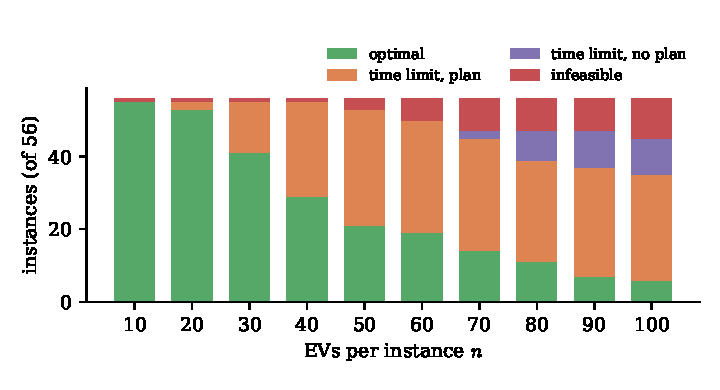
\includegraphics[width=0.66\textwidth]{figures/solver_outcome.pdf}
\caption{Outcome of the 56 instances of each size.}
\label{fig:solver}
\end{figure}
\begin{table}[H]
\centering\small
\caption{Solver outcome per instance size; gap of the time-limit plans.}
\label{tab:solver}
\begin{tabular}{@{}rrrrrrrr@{}}
\toprule
$n$ & instances & optimal & \shortstack[r]{time limit\\with plan} & \shortstack[r]{time limit\\no plan} & infeasible & \shortstack[r]{median\\gap (\%)} & \shortstack[r]{mean\\time (s)} \\
\midrule
10 & 56 & 55 & 0 & 0 & 1 & -- & 0 \\
20 & 56 & 53 & 2 & 0 & 1 & 1.02 & 23 \\
30 & 56 & 41 & 14 & 0 & 1 & 1.88 & 96 \\
40 & 56 & 29 & 26 & 0 & 1 & 3.66 & 154 \\
50 & 56 & 21 & 32 & 0 & 3 & 5.91 & 182 \\
60 & 56 & 19 & 31 & 0 & 6 & 7.54 & 186 \\
70 & 56 & 14 & 31 & 2 & 9 & 6.98 & 191 \\
80 & 56 & 11 & 28 & 8 & 9 & 3.53 & 218 \\
90 & 56 & 7 & 30 & 10 & 9 & 2.13 & 236 \\
100 & 56 & 6 & 29 & 10 & 11 & 2.76 & 221 \\
\midrule
all & 560 & 256 & 223 & 30 & 51 & 4.22 & 151 \\
\bottomrule
\end{tabular}

\end{table}
Small instances are solved to optimality almost always (55 of 56 at $n=10$). From $n=40$ on, most instances end at the time limit with a good plan (median gap \GapMed\pct). Infeasible instances appear from $n=10$ in RC1 and from $n=50$ in R1; instances with no plan at all appear from $n=70$.

\inshort{\NOpt{} optimal, \NTL{} time-limit plans, \NNone{} unsolved, \NInf{} infeasible; all \NValid{} plans valid.}

\subsection{Instance-level overview}
\begin{table}[H]
\centering\footnotesize
\caption{Distribution of instance-level results over the valid plans.}
\label{tab:inststats}
\begin{tabular}{@{}lrrrrrrr@{}}
\toprule
measure (per instance) & count & mean & median & 10th pct & 90th pct & min & max \\
\midrule
objective $Z$ per EV (Rs) & 479 & 938 & 917 & 849 & 1070 & 812 & 1233 \\
operator share of $Z$ (\%) & 479 & 30.0 & 29.0 & 26.5 & 36.6 & 19.9 & 50.2 \\
vans used & 479 & 2.2 & 2.0 & 1.0 & 4.0 & 0.0 & 5.0 \\
EVs served by a van (\%) & 479 & 22.0 & 20.0 & 15.0 & 30.0 & 0.0 & 60.0 \\
free-choice EVs by van (\%) & 479 & 8.0 & 6.5 & 0.0 & 16.7 & 0.0 & 55.6 \\
mean FCS queue (min) & 479 & 0.99 & 0.00 & 0.00 & 4.31 & 0.00 & 11.92 \\
mean van wait (min) & 472 & 23.9 & 17.7 & 0.0 & 62.1 & 0.0 & 118.5 \\
mean request to charged (min) & 479 & 63.1 & 59.3 & 54.2 & 77.1 & 44.9 & 111.0 \\
van km & 479 & 71.2 & 73.6 & 25.5 & 119.8 & 0.0 & 201.8 \\
solver time (s), all instances & 560 & 151 & 110 & 0 & 300 & 0 & 317 \\
gap of time-limit plans (\%) & 223 & 6.60 & 4.22 & 0.71 & 16.87 & 0.04 & 26.89 \\
\bottomrule
\end{tabular}

\end{table}
\begin{figure}[H]
\centering
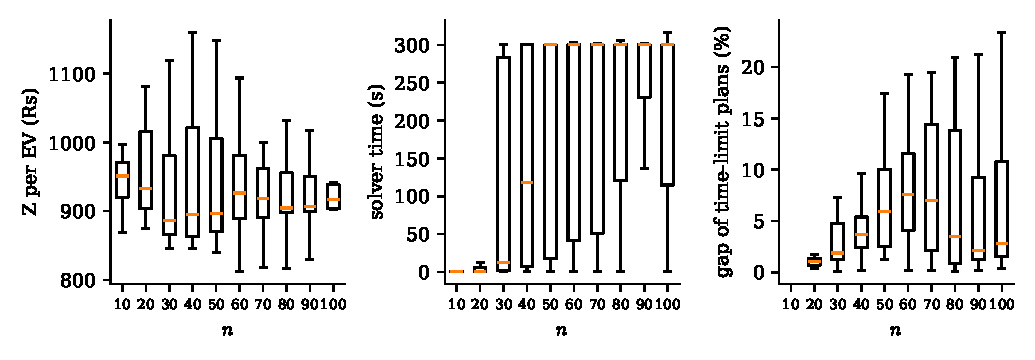
\includegraphics[width=\textwidth]{figures/c_inst_by_n.pdf}
\caption{Objective per EV, solver time and gap by instance size (boxes: middle 50\pct, line: median).}
\label{fig:instn}
\end{figure}
\begin{itemize}
  \item The objective per EV is fairly stable: \ZperMean{} Rs on average, between \ZperMin{} and \ZperMax{} Rs. It falls slightly with $n$ because the fixed van dispatch cost is shared by more EVs.
  \item About 2 vans leave per instance and serve about a fifth of the EVs (22\pct{} on average); most of them are the stranded EVs, who are 15\pct{} of all EVs.
  \item Solver time reaches the 300\,s limit from $n\approx40$; the gaps of time-limit plans are small (median \GapMed\pct).
\end{itemize}

\subsection{Families}
\begin{table}[H]
\centering\footnotesize
\caption{Results by Solomon family.}
\label{tab:family}
\begin{tabular}{@{}lrrrrrrrrr@{}}
\toprule
family & instances & valid plans & \shortstack[r]{Z per EV\\(Rs)} & \shortstack[r]{operator\\share (\%)} & \shortstack[r]{free-choice\\by van (\%)} & \shortstack[r]{mean queue\\(min)} & \shortstack[r]{request to\\charged (min)} & \shortstack[r]{vans\\used} & $T$ (min) \\
\midrule
C1 & 90 & 90 & 920 & 29.7 & 6.9 & 0.86 & 63.4 & 2.14 & 1236 \\
C2 & 80 & 79 & 929 & 29.3 & 8.9 & 0.86 & 62.5 & 1.94 & 3390 \\
R1 & 120 & 76 & 919 & 32.4 & 5.6 & 2.29 & 60.1 & 2.38 & 230 \\
R2 & 110 & 110 & 871 & 29.8 & 5.9 & 1.72 & 62.4 & 2.02 & 1000 \\
RC1 & 80 & 44 & 1064 & 28.5 & 7.8 & 2.44 & 76.0 & 2.39 & 240 \\
RC2 & 80 & 80 & 1009 & 29.7 & 7.2 & 0.91 & 66.0 & 2.31 & 960 \\
\bottomrule
\end{tabular}

\end{table}
\begin{figure}[H]
\centering
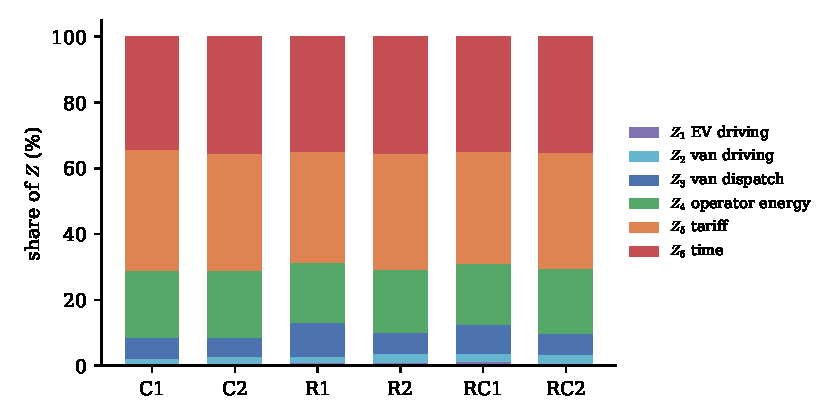
\includegraphics[width=0.75\textwidth]{figures/c_obj_family.pdf}
\caption{Composition of the objective by family.}
\label{fig:objfamily}
\end{figure}
The short-horizon families R1 and RC1 have the fewest valid plans (76 of 120 and 44 of 80): their horizon of 230--240 minutes leaves little room. RC families have the highest cost per EV (longer distances). The composition of $Z$ is almost the same in every family: about 30\pct{} operator cost and 70\pct{} perceived customer cost.

\inshort{Families differ mainly in how often a plan exists (short horizons) and in cost level (RC dearer); the cost structure is the same everywhere.}

\subsection{EV-level distributions}
\begin{table}[H]
\centering\footnotesize
\caption{Distribution of EV-level variables (all EVs of valid plans unless stated).}
\label{tab:evstats}
\begin{tabular}{@{}lrrrrrr@{}}
\toprule
variable (per EV) & count & mean & median & 10th pct & 90th pct & max \\
\midrule
income $\theta$ & 24250 & 0.50 & 0.51 & 0.18 & 0.81 & 0.98 \\
energy demand $E_i$ (kWh) & 24250 & 19.6 & 19.2 & 14.3 & 27.8 & 40.0 \\
nearest reachable FCS (km) & 20584 & 1.61 & 1.50 & 0.65 & 2.70 & 4.71 \\
demand pressure & 20584 & 0.48 & 0.21 & 0.03 & 1.38 & 2.66 \\
drive to FCS (km), FCS users & 19147 & 2.28 & 1.63 & 0.66 & 4.45 & 22.84 \\
FCS queue (min), FCS users & 19147 & 1.37 & 0.00 & 0.00 & 0.00 & 55.75 \\
van wait (min), van users & 5103 & 26.5 & 0.0 & 0.0 & 89.2 & 379.6 \\
charging time (min) & 24250 & 50.7 & 44.0 & 31.0 & 75.7 & 109.1 \\
request to charged (min) & 24250 & 64.2 & 59.9 & 38.7 & 95.6 & 435.1 \\
money paid (Rs) & 24250 & 341 & 327 & 234 & 511 & 1000 \\
perceived money (Rs) & 24250 & 338 & 317 & 195 & 504 & 1000 \\
perceived time (Rs) & 24250 & 328 & 302 & 116 & 552 & 1771 \\
perceived total (Rs) & 24250 & 666 & 630 & 433 & 962 & 2074 \\
\bottomrule
\end{tabular}

\end{table}
\begin{figure}[H]
\centering
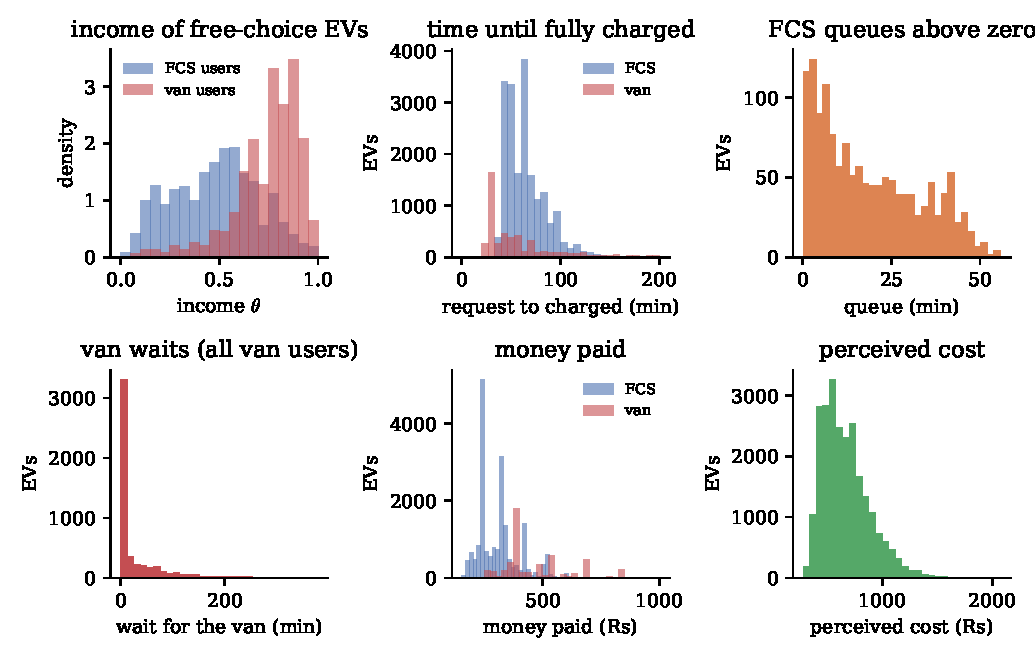
\includegraphics[width=\textwidth]{figures/c_ev_dists.pdf}
\caption{Distributions of income, time until charged, queues, van waits, money paid and perceived cost.}
\label{fig:evdists}
\end{figure}
\begin{itemize}
  \item Van users are much richer than station users (top left). Most EVs are fully charged within about 40--95 minutes of their request (10th to 90th percentile); van users with short waits are charged fastest (30\,kW against 22\,kW).
  \item Only \NQueued{} of the \NFCSfree{} free-choice station users queue at all; their queues spread up to about 55 minutes.
  \item Most van users are served with no wait, but there is a long tail; Section~\ref{sec:choice} shows that the longest waits belong to plans that were not proven optimal.
  \item Money paid clusters by energy demand; van users pay more because $p^{\mathrm M}>p^{\mathrm F}$.
\end{itemize}

\subsection{Correlations}
\begin{figure}[H]
\centering
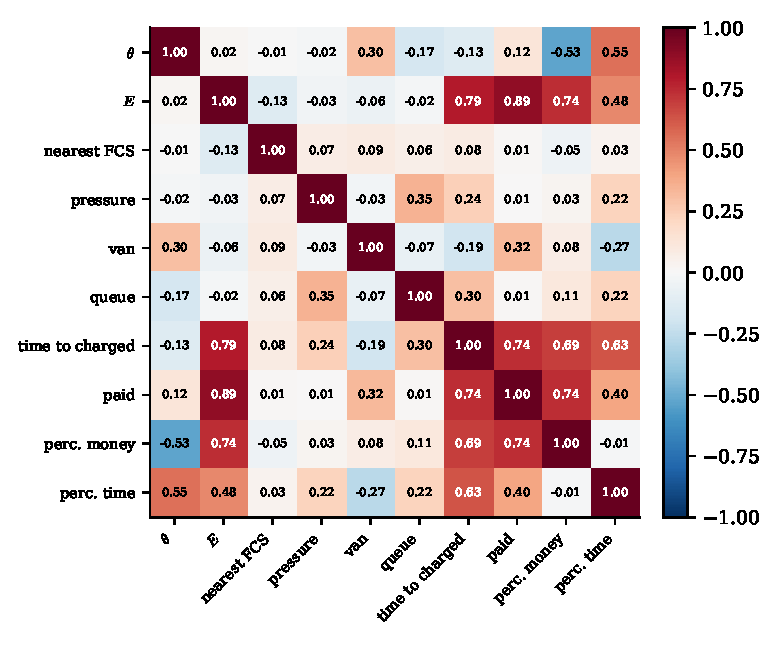
\includegraphics[width=0.62\textwidth]{figures/c_corr.pdf}
\caption{Spearman correlations between EV-level variables (free-choice EVs).}
\label{fig:corr}
\end{figure}
Income is the variable most correlated with being served by a van ($\rho=\CorrThetaVan$) and is negatively correlated with queueing ($\rho=\CorrThetaQueue$) and with the time until charged ($\rho=\CorrThetaTime$). Demand pressure is the strongest correlate of queueing ($\rho=\CorrPressQueue$). Money paid is driven by the energy demand ($\rho=\CorrEPay$).

\inshort{Income goes with vans, short queues and fast charging; demand pressure goes with queues; energy goes with money paid.}

%=====================================================================
\clearpage
\part{Comprehensive analysis}
\section{Analysis point by point}

%---------------------------------------------------------------------
\subsection{Anatomy of the objective function}
\label{sec:anatomy}

\subsubsection{The six terms}
\[
Z=\underbrace{Z_1}_{\substack{\text{EV driving}\\\mu_i c^{\mathrm{EV}} d_{if}}}+\underbrace{Z_2}_{\substack{\text{van driving}\\ c^{\mathrm M}\,\text{km}}}+\underbrace{Z_3}_{\substack{\text{dispatch}\\ c^{\mathrm F}_m u_m}}+\underbrace{Z_4}_{\substack{\text{energy}\\ \pi^{\mathrm F}E_i,\ \pi^{\mathrm M}E_i/\eta}}+\underbrace{Z_5}_{\substack{\text{tariff}\\ \mu_i p E_i}}+\underbrace{Z_6}_{\substack{\text{time}\\ c^{a}_i\times\text{minutes}}}
\]
$Z_2+Z_3+Z_4$ is the operator's cost (\ZOperator\pct{} of $Z$ over all valid plans) and $Z_1+Z_5+Z_6$ the customers' perceived cost (\ZCustomer\pct). The largest single terms are the perceived tariff $Z_5$ (\ZFive\pct) and perceived time $Z_6$ (\ZSix\pct), then operator energy $Z_4$ (\ZFour\pct), van dispatch $Z_3$ (\ZThree\pct), van driving $Z_2$ (\ZTwo\pct) and EV driving $Z_1$ (\ZOne\pct). Only $Z_1$, $Z_5$ and $Z_6$ depend on income.

\subsubsection{How sensitive is $Z$ to each coefficient? (envelope theorem)}
Every term of $Z$ is a coefficient times a quantity of the plan (km, kWh, minutes, vans). Write the optimal objective as $Z^{*}(c)=\min_{x}\sum_k c_k\,g_k(x)$. The \emph{envelope theorem} says that, as long as the optimal plan $x^{*}$ does not change,
\[
\frac{\partial Z^{*}}{\partial c_k}=g_k(x^{*}),\qquad
\text{elasticity}_k=\frac{c_k}{Z^{*}}\frac{\partial Z^{*}}{\partial c_k}=\frac{c_k\,g_k(x^{*})}{Z^{*}}=\text{share of }Z\text{ carried by }c_k .
\]
So the elasticity of $Z$ with respect to a coefficient is simply the share of the objective that coefficient multiplies. Because $Z^{*}(c)$ is a minimum of linear functions of $c$, it is \emph{concave}: after re-optimising, the true $Z^{*}$ is never above the linear prediction $Z^{*}+g_k(x^{*})\Delta c_k$. The table is therefore an upper bound on how much $Z$ can rise.

\begin{table}[H]
\centering\footnotesize
\caption{Derivative and elasticity of $Z$ with respect to every coefficient (all valid plans). The income coefficients are the end points of the straight lines: $\mu^{0}$ is the money sensitivity at $\theta=0$, $c^{\mathrm{C},1}$ the value of FCS charging time at $\theta=1$, and so on.}
\label{tab:elasticity}
\begin{tabular}{@{}lrlrrr@{}}
\toprule
coefficient & value & meaning & \shortstack[r]{$\partial Z/\partial$coef.\\per plan} & \shortstack[r]{elasticity\\(\%)} & \shortstack[r]{Rs per plan\\for +10\%} \\
\midrule
$c^{\mathrm{EV}}$ & 4 & EV driving cost (Rs/km) & 96.4 & 0.81 & 39 \\
$c^{\mathrm M}$ & 15 & van driving cost (Rs/km) & 71.2 & 2.26 & 107 \\
$c^{\mathrm F}_m$ & 1500 & van dispatch cost (Rs) & 2.2 & 6.88 & 325 \\
$\pi^{\mathrm F}$ & 8.7 & grid energy at FCS (Rs/kWh) & 794.2 & 14.61 & 691 \\
$\pi^{\mathrm M}$ & 10.7 & van battery energy (Rs/kWh) & 221.8 & 5.02 & 237 \\
$p^{\mathrm F}$ & 15 & FCS tariff (Rs/kWh) & 809.5 & 25.67 & 1214 \\
$p^{\mathrm M}$ & 25 & van tariff (Rs/kWh) & 183.2 & 9.68 & 458 \\
$\mu^{0}$ & 1.5 & money sensitivity at $\theta=0$ & 8474.8 & 26.87 & 1271 \\
$\mu^{1}$ & 0.5 & money sensitivity at $\theta=1$ & 8792.6 & 9.29 & 440 \\
$c^{\mathrm{D},0}$ & 1.5 & value of time, driving, $\theta=0$ & 195.5 & 0.62 & 29 \\
$c^{\mathrm{D},1}$ & 15 & value of time, driving, $\theta=1$ & 155.0 & 4.91 & 233 \\
$c^{\mathrm{Q},0}$ & 2.5 & value of time, queueing, $\theta=0$ & 38.6 & 0.20 & 10 \\
$c^{\mathrm{Q},1}$ & 25 & value of time, queueing, $\theta=1$ & 16.2 & 0.86 & 41 \\
$c^{\mathrm{C},0}$ & 1 & value of time, FCS charging, $\theta=0$ & 1124.7 & 2.38 & 112 \\
$c^{\mathrm{C},1}$ & 10 & value of time, FCS charging, $\theta=1$ & 1041.3 & 22.01 & 1041 \\
$c^{\mathrm{V},0}$ & 0.5 & value of time, van wait + charging, $\theta=0$ & 326.0 & 0.34 & 16 \\
$c^{\mathrm{V},1}$ & 5 & value of time, van wait + charging, $\theta=1$ & 355.0 & 3.75 & 177 \\
\bottomrule
\end{tabular}

\end{table}
\begin{figure}[H]
\centering
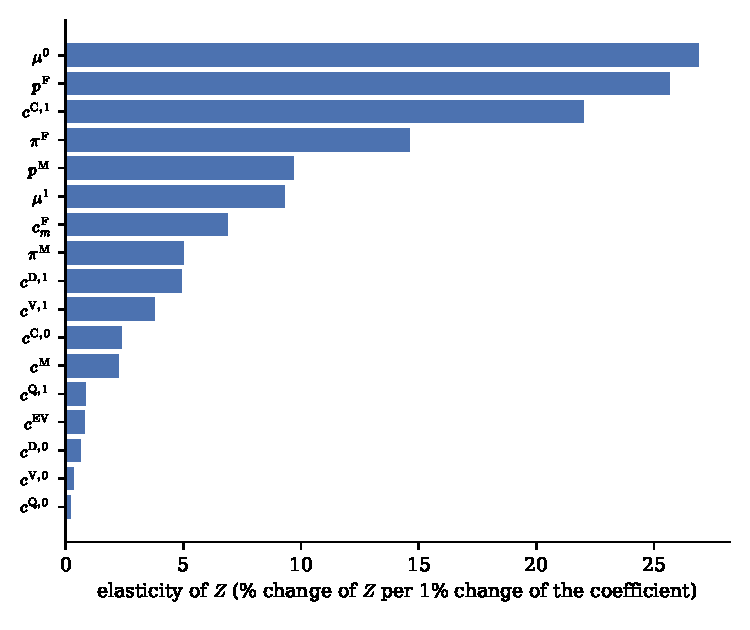
\includegraphics[width=0.62\textwidth]{figures/c_elasticity.pdf}
\caption{Elasticity of $Z$ with respect to each coefficient.}
\label{fig:elasticity}
\end{figure}
\begin{itemize}
  \item The most influential coefficients are the station tariff $p^{\mathrm F}$ (elasticity \ElPF\pct), the money sensitivity of the poorest $\mu^{0}$ (\ElMuZero\pct), the value of station-charging time of the richest $c^{\mathrm{C},1}$ (\ElCCOne\pct) and the grid price $\pi^{\mathrm F}$ (\ElPiF\pct). A 10\pct{} rise of $p^{\mathrm F}$ would raise $Z$ by at most about 2.6\pct.
  \item Queueing coefficients matter little in total ($c^{\mathrm{Q},0}$: \ElCQZero\pct, $c^{\mathrm{Q},1}$: \ElCQOne\pct) because few EVs queue; they matter a lot \emph{locally}, for who queues (Section~\ref{sec:queues}).
  \item Groups add up: operator coefficients $c^{\mathrm M},c^{\mathrm F},\pi^{\mathrm F},\pi^{\mathrm M}$ together \ElOperator\pct; the money sensitivities $\mu^{0}+\mu^{1}$ together \ElMoney\pct, the same as the tariffs and the EV driving cost together (\ElTariffs\pct), because the money terms are products $\mu\times p$; all value-of-time end points together \ElTime\pct.
  \item The dispatch cost $c^{\mathrm F}$ has a small total elasticity (\ElCF\pct) but a large effect on decisions: it decides when a van leaves at all (Section~\ref{sec:threshold}).
\end{itemize}

\inshort{About 70\pct{} of $Z$ is what customers feel and 30\pct{} what the operator pays. The station tariff, the money sensitivity of low incomes, the value of charging time of high incomes and the grid price move $Z$ most; these elasticities are upper bounds because the plan can adapt.}

%---------------------------------------------------------------------
\subsection{Duality and shadow prices}
\label{sec:duals}

\subsubsection{Recap: duality in linear programming}
For a linear program in minimisation form
\[
\text{(P)}\quad \min\ c^{\top}x\ \ \text{s.t. } Ax\ge b,\ x\ge0
\qquad\Longleftrightarrow\qquad
\text{(D)}\quad \max\ b^{\top}y\ \ \text{s.t. } A^{\top}y\le c,\ y\ge0 ,
\]
strong duality gives equal optima, and the optimal dual value $y_k$ of constraint $k$ is its \emph{shadow price}: $y_k=\partial z^{*}/\partial b_k$, the change of the optimal cost when the right-hand side $b_k$ grows by one unit. \emph{Complementary slackness} says that a constraint with slack has $y_k=0$, and only binding constraints can have a non-zero price. The economic reading (course lecture 11): $y_k$ is what one more unit of the resource behind constraint $k$ is worth.

\subsubsection{Why a MILP has no duals, and what we do instead}
In a MILP the 0/1 variables make the feasible set non-convex, so there is no dual in the LP sense, and the duals of the LP relaxation describe a fractional problem with weak big-$M$ constraints, not our plans. The standard remedy is the \emph{fixed-plan LP}: keep every yes/no decision of the plan (resource of each EV, order on each gun, every van route) and re-solve only the continuous part, the start times $S_i$ and the waits $q^{\mathrm F}_i$, $q^{\mathrm M}_i$:
\begin{align*}
\min\ & \textstyle\sum_{i\in\text{FCS}} c^{\mathrm Q}_i q^{\mathrm F}_i+\sum_{i\in\text{van}} c^{\mathrm V}_i q^{\mathrm M}_i\\
\text{FCS user } i:\ & S_i\ge r_i+t_{if},\quad q^{\mathrm F}_i=S_i-r_i-t_{if},\quad q^{\mathrm F}_i\le W_i,\quad S_i\le T-\tau^{\mathrm F}_i\\
i\text{ then }j\text{ on a gun}:\ & S_j\ge S_i+\tau^{\mathrm F}_i\\
\text{van user } i:\ & S_i\ge r_i,\quad q^{\mathrm M}_i=S_i-r_i,\quad S_i\le T-\tau^{\mathrm M}_i\\
\text{van route } 0\to a\to\dots\to b\to0:\ & S_a\ge t_{0a},\quad S_j\ge S_i+\tau^{\mathrm M}_i+t_{ij},\quad S_b\le T-\tau^{\mathrm M}_b-t_{b0}.
\end{align*}
Everything else in $Z$ (energy, tariffs, driving, dispatch, charging time) is constant once the decisions are fixed. The duals of this LP are the shadow prices \emph{of the plan}: what one more unit would be worth if the decisions stayed as they are. We solved it for all \NValid{} plans. \textbf{Check:} in every plan the LP optimum equals the plan's own waiting cost, so the LP reproduces the plans exactly.

\begin{table}[H]
\centering\footnotesize
\caption{Shadow prices of the fixed-plan LPs, all valid plans (absolute values).}
\label{tab:duals}
\begin{tabular}{@{}lrrrrrp{4.6cm}@{}}
\toprule
constraint & rows & \shortstack[r]{non-zero\\dual (\%)} & \shortstack[r]{mean\\(Rs/min)} & \shortstack[r]{median\\(Rs/min)} & \shortstack[r]{max\\(Rs/min)} & meaning of the dual \\
\midrule
FCS arrival $S_i\ge r_i+t_{if}$ & 19147 & 7.7 & 11.51 & 10.40 & 44.15 & not unique (degenerate, Section 4.2.7); not interpreted \\
van release $S_i\ge r_i$ & 5103 & 52.7 & 3.80 & 3.69 & 17.35 & not unique (degenerate); not interpreted \\
gun order $S_j\ge S_i+\tau^{\mathrm F}_i$ & 10903 & 13.0 & 11.63 & 10.40 & 44.15 & value of one gun-minute: delay EV $i$ passes to those behind it \\
van order $S_j\ge S_i+\tau^{\mathrm M}_i+t_{ij}$ & 4064 & 40.6 & 4.50 & 3.96 & 18.31 & value of one van-minute on that leg \\
first stop $S_a\ge t_{0a}$ & 1039 & 73.1 & 7.36 & 6.66 & 21.41 & value of an earlier van departure \\
queue limit $q^{\mathrm F}_i\le W_i$ & 19147 & 0.0 & 0.00 & 0.00 & 0.00 & value of one more minute of patience \\
deadline $C_i\le T$, van return & 25289 & 0.0 & 0.00 & 0.00 & 0.00 & value of one more minute of horizon \\
\bottomrule
\end{tabular}

\end{table}

\subsubsection{Gun-minutes: the price of congestion}
The dual of a gun-order constraint $S_j\ge S_i+\tau^{\mathrm F}_i$ is the value of one gun-minute at that moment: if EV $i$ held the gun one minute less, EV $j$ and everyone queued behind $j$ would start one minute earlier, and $Z$ would fall by the sum of their queueing rates $c^{\mathrm Q}$. It is the \emph{congestion externality} that EV $i$ imposes on the EVs behind it.
\begin{figure}[H]
\centering
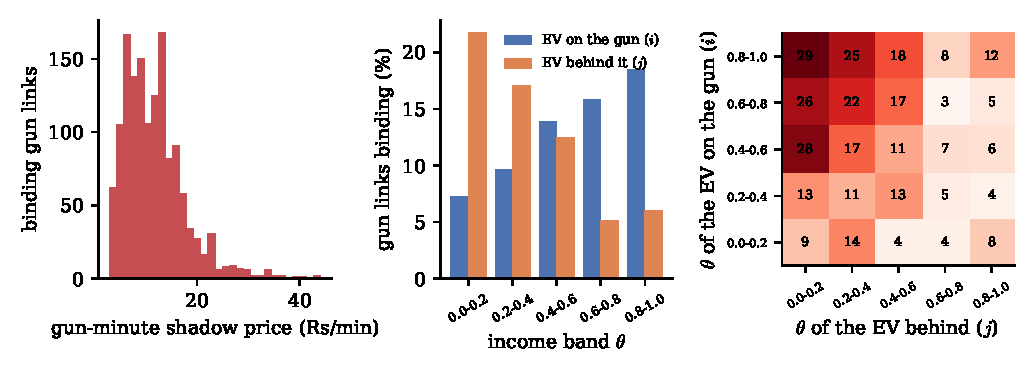
\includegraphics[width=\textwidth]{figures/c_gun_duals.pdf}
\caption{Left: gun-minute shadow prices where they are non-zero. Middle: share of binding gun links by income of the EV on the gun and of the EV behind it. Right: share binding (\%) by the income of both.}
\label{fig:gunduals}
\end{figure}
\begin{table}[H]
\centering\small
\caption{Gun links by demand pressure of the EV behind.}
\label{tab:gunpressure}
\begin{tabular}{@{}lrrrr@{}}
\toprule
\shortstack[l]{demand pressure\\of the follower} & gun links & \shortstack[r]{binding\\(\%)} & \shortstack[r]{mean dual if\\binding (Rs/min)} & \shortstack[r]{mean dual\\all links (Rs/min)} \\
\midrule
low & 5471 & 0.5 & 11.7 & 0.06 \\
medium & 3254 & 2.2 & 13.2 & 0.29 \\
high & 2178 & 60.3 & 11.5 & 6.96 \\
\bottomrule
\end{tabular}

\end{table}
\begin{itemize}
  \item Of \GunRows{} consecutive gun links, \GunBind\pct{} are binding. Where binding, a gun-minute is worth \GunMean{} Rs on average (median \GunMed, up to \GunMax{} Rs/min).
  \item Congestion is a peak phenomenon: \GunBindHigh\pct{} of gun links are binding when the EV behind arrives at high demand pressure, against \GunBindLow\pct{} at low pressure.
  \item \textbf{Who imposes the externality and who bears it.} A gun link is binding in \GunOccTop\pct{} of the cases when the EV on the gun is in the richest band and \GunOccBot\pct{} when it is in the poorest. Seen from the EV behind it is the reverse: \GunFolBot\pct{} for the poorest and \GunFolTop\pct{} for the richest. The heat map shows the pattern: the darkest cells are a rich EV on the gun and a poor EV waiting.
  \item This is the queue priority of Section~\ref{sec:queues} in dual form: the model lets the customer with the higher value of time go first, because the waiting EV's queueing rate $c^{\mathrm Q}(\theta)$ is lower.
\end{itemize}

\subsubsection{Van-minutes}
The dual of a van-order constraint is the value of one van-minute on that leg: \VanBind\pct{} of van legs are binding, worth \VanMean{} Rs/min on average when binding. Van-minutes are cheaper than gun-minutes because the EVs waiting for a van feel only the driver-free rate $c^{\mathrm V}$.

\subsubsection{Patience limits and the deadline: zero shadow prices}
All \PatRows{} queue-limit constraints $q^{\mathrm F}_i\le W_i$ and all \DeadRows{} deadline and van-return constraints have shadow price zero in every plan, so $\partial Z/\partial T=0$ and $\partial Z/\partial W_i=0$ for every fixed plan. By complementary slackness none of them is binding: no station user queues up to its limit and no EV finishes exactly at $T$ in a way that delays others. These constraints still matter, but only through the \emph{decisions}: they rule out plans (a queue longer than $W_i$, a van route too long for $T$), and the 51 infeasible instances exist only because of the deadline. A fixed-plan LP cannot see that; measuring it would need re-solving the MILP with a longer $T$ or a larger $W$.

\subsubsection{The value of charger power}
The charging times depend on power: $\tau^{\mathrm F}_i=60E_i/P^{\mathrm F}$ and $\tau^{\mathrm M}_i=60E_i/P^{\mathrm M}$. By the chain rule, with the decisions fixed,
\[
\frac{\partial Z}{\partial P^{\mathrm F}}=\sum_{i\in\text{FCS}}\Big(c^{\mathrm C}_i+\lambda^{\text{gun}}_{i}-\lambda^{\text{deadline}}_{i}\Big)\frac{\partial\tau^{\mathrm F}_i}{\partial P^{\mathrm F}},\qquad\frac{\partial\tau^{\mathrm F}_i}{\partial P^{\mathrm F}}=-\frac{\tau^{\mathrm F}_i}{P^{\mathrm F}},
\]
where $c^{\mathrm C}_i$ is the customer's own charging-time rate and $\lambda^{\text{gun}}_i$ the gun-minute price behind EV $i$.
\begin{figure}[H]
\centering
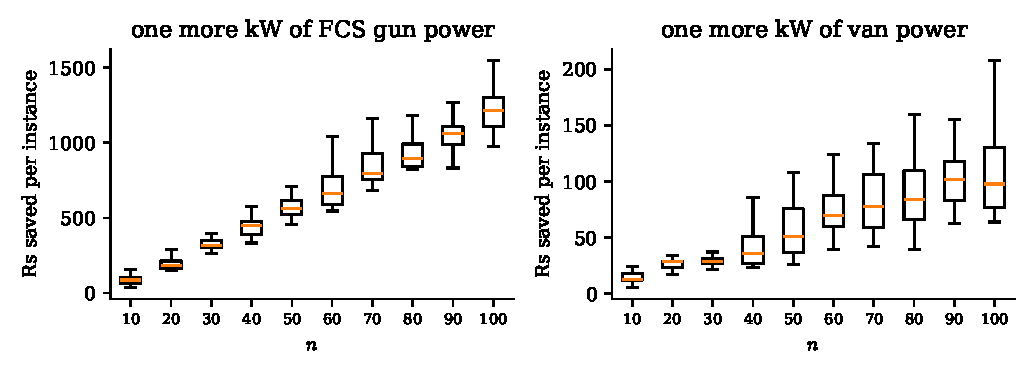
\includegraphics[width=0.85\textwidth]{figures/c_power_value.pdf}
\caption{Value of one more kW of charging power per instance, by instance size.}
\label{fig:power}
\end{figure}
One more kW of station-gun power (22 to 23\,kW) is worth \DPFmean{} Rs per instance on average (median \DPFmed, up to \DPFmax), about \DPFperEV{} Rs per EV. \DPFcong\pct{} of it is congestion relief (shorter queues for the EVs behind), the rest is the customers' own shorter charging time. One more kW of van power is worth \DPMmean{} Rs per instance (up to \DPMmax). Faster station guns are worth about ten times more than faster vans, because far more EVs charge at stations.

\subsubsection{What these shadow prices cannot tell}
\begin{itemize}
  \item They hold for the given decisions. Discrete resources (one more van, one more gun, one more seat $Q_m$, a larger battery) change the decisions and need re-solving the MILP; their constraints are constants in the fixed-plan LP.
  \item The duals of the arrival and release constraints are not unique: when an EV starts the moment it arrives, both its arrival constraint and its zero-wait bound are binding (degenerate), and the solver may split the price between them. We report but do not interpret them.
\end{itemize}

\inshort{Fixing each plan's decisions gives an exact LP whose duals are the plan's shadow prices. Gun-minutes are the scarce resource at peak (\GunMean{} Rs/min when binding), and the price is paid by poorer customers waiting behind richer ones. Patience limits and the deadline have zero marginal value; they act only by excluding plans. One more kW at the stations is worth about \DPFmean{} Rs per instance.}

%---------------------------------------------------------------------
\subsection{The income threshold: theory against data}
\label{sec:threshold}

\subsubsection{The formula}
Section 4.1 of the formulation compares, for one EV with everything else fixed, the cost of a van with the cost of its station:
\[
\Delta_i(\theta)=\mu(\theta)\big[(p^{\mathrm M}-p^{\mathrm F})E_i-c^{\mathrm{EV}}d_{if}\big]+\kappa_i-c^{\mathrm D}(\theta)t_{if}-c^{\mathrm Q}(\theta)q^{\mathrm F}_i-c^{\mathrm C}(\theta)\tau^{\mathrm F}_i+c^{\mathrm V}(\theta)\big(q^{\mathrm M}_i+\tau^{\mathrm M}_i\big),
\]
with $\kappa_i=(\pi^{\mathrm M}/\eta-\pi^{\mathrm F})E_i+c^{\mathrm M}x_i$ ($x_i$ = extra van km) $+\,c^{\mathrm F}$ if the van would not leave otherwise. The van is chosen when $\Delta_i<0$; with straight-line sensitivities $\Delta_i$ is linear in $\theta$, so there is one threshold $\theta^{*}_i$ with $\Delta_i(\theta^{*}_i)=0$.

\subsubsection{The numbers for a typical EV}
Take $E=20$\,kWh, 2\,km to the nearest station ($t=7.7$\,min), no station queue, a 10-minute van wait and a 4\,km van detour. Then $\tau^{\mathrm F}=54.5$\,min, $\tau^{\mathrm M}=40$\,min, the money bracket is $10\cdot20-4\cdot2=192$\,Rs and $\kappa=\KappaTypical$\,Rs:
\[
\Delta(\theta)=\mu(\theta)\cdot192+124-c^{\mathrm D}(\theta)\cdot7.7-c^{\mathrm C}(\theta)\cdot54.5+c^{\mathrm V}(\theta)\cdot50,\qquad
\Delta(0)=\DeltaZero,\quad \Delta(1)=\DeltaOne\ \text{Rs},
\]
so $\theta^{*}=\DeltaZero/(\DeltaZero+191)=\ThetaStar$.

\begin{figure}[H]
\centering
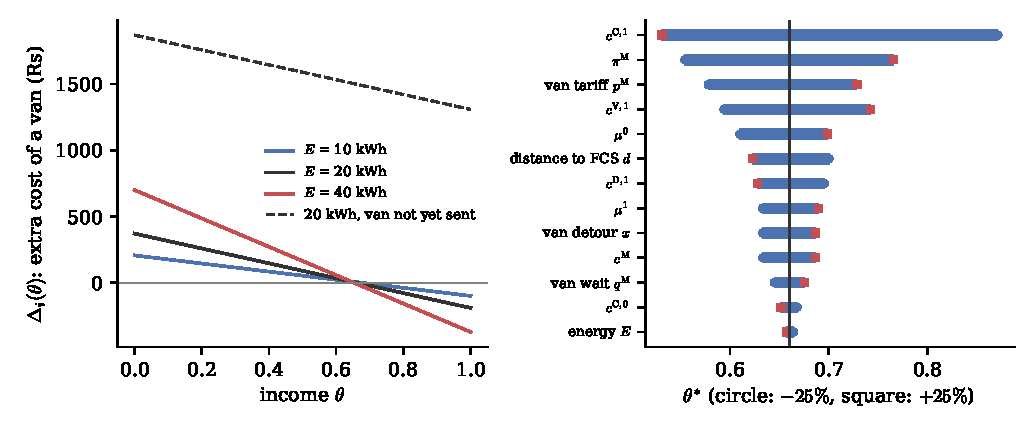
\includegraphics[width=\textwidth]{figures/c_threshold.pdf}
\caption{Left: extra cost of a van $\Delta(\theta)$ for three energy demands, and with the van's dispatch cost (dashed). Right: how $\theta^{*}$ moves when each parameter changes by $\pm25\%$.}
\label{fig:threshold}
\end{figure}
\begin{figure}[H]
\centering
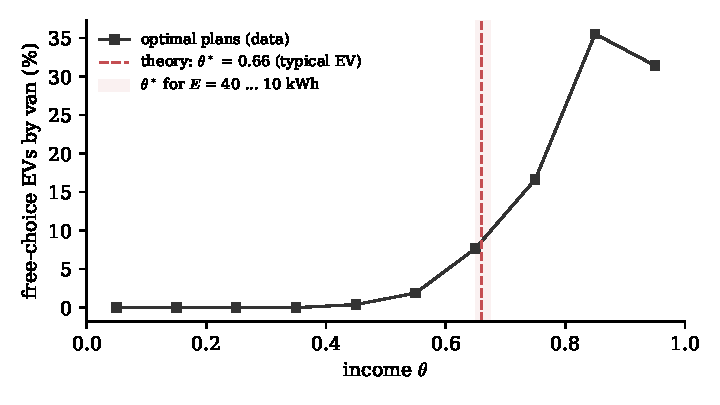
\includegraphics[width=0.66\textwidth]{figures/c_threshold_data.pdf}
\caption{Theory against data: van share of free-choice EVs in optimal plans and the predicted threshold.}
\label{fig:thresholddata}
\end{figure}
\begin{table}[H]
\centering\small
\caption{Threshold $\theta^{*}$ of the typical EV when one parameter changes by $\pm25\%$, sorted by swing.}
\label{tab:tornado}
\begin{tabular}{@{}lrrrr@{}}
\toprule
parameter ($\pm25\%$) & $\theta^{*}$ at $-25\%$ & $\theta^{*}$ base & $\theta^{*}$ at $+25\%$ & swing \\
\midrule
$c^{\mathrm{C},1}$ & 0.87 & 0.66 & 0.53 & 0.34 \\
$\pi^{\mathrm M}$ & 0.55 & 0.66 & 0.77 & 0.21 \\
van tariff $p^{\mathrm M}$ & 0.58 & 0.66 & 0.73 & 0.15 \\
$c^{\mathrm{V},1}$ & 0.59 & 0.66 & 0.74 & 0.15 \\
$\mu^{0}$ & 0.61 & 0.66 & 0.70 & 0.09 \\
distance to FCS $d$ & 0.70 & 0.66 & 0.62 & 0.08 \\
$c^{\mathrm{D},1}$ & 0.70 & 0.66 & 0.63 & 0.07 \\
$\mu^{1}$ & 0.63 & 0.66 & 0.69 & 0.06 \\
$c^{\mathrm M}$ & 0.63 & 0.66 & 0.69 & 0.05 \\
van detour $x$ & 0.63 & 0.66 & 0.69 & 0.05 \\
van wait $q^{\mathrm M}$ & 0.64 & 0.66 & 0.68 & 0.03 \\
$c^{\mathrm{C},0}$ & 0.67 & 0.66 & 0.65 & 0.02 \\
energy $E$ & 0.66 & 0.66 & 0.66 & 0.01 \\
\bottomrule
\end{tabular}

\end{table}

\subsubsection{What the threshold explains}
\begin{itemize}
  \item \textbf{Theory meets data.} The van share in optimal plans is near zero below $\theta\approx0.5$ and jumps between 0.6 and 0.8; the predicted $\theta^{*}=\ThetaStar$ sits exactly at the jump (Figure~\ref{fig:thresholddata}). The step in the data is the formulation's own trade-off at work, not an accident of the solver.
  \item \textbf{Vans leave for the stranded, the rich fill the seats.} If the van must be sent out for this EV alone, $\Delta$ includes the dispatch cost $c^{\mathrm F}=1500$\,Rs and stays positive at every income ($\Delta(1)=\DeltaDispatchOne$\,Rs, $\theta^{*}=\ThetaStarDispatch$). No free-choice customer ever justifies a van alone; vans leave for the stranded EVs, and their spare seats go to the high-income customers.
  \item \textbf{Queues lower the threshold, van waits raise it.} A 10-minute station queue lowers $\theta^{*}$ to \ThetaStarQueue; a 40-minute van wait raises it to \ThetaStarWait.
  \item \textbf{Distance matters, energy barely does.} An EV 5\,km from its station has $\theta^{*}=\ThetaStarFar$, one at 0.5\,km \ThetaStarNear. The energy demand hardly moves $\theta^{*}$ (\ThetaStarBigE{} at 40\,kWh, \ThetaStarSmallE{} at 10\,kWh): the van premium and the charging time saved both grow in proportion to $E$.
  \item \textbf{Which parameters move the threshold most.} The value of station-charging time of the rich $c^{\mathrm{C},1}$ (swing 0.34 for $\pm25\%$), the van energy price $\pi^{\mathrm M}$, the van tariff $p^{\mathrm M}$ and the driver-free value of time of the rich $c^{\mathrm{V},1}$. These are the parameters to calibrate first.
\end{itemize}

\inshort{The formulation predicts $\theta^{*}=\ThetaStar$ for a typical EV, and the optimal plans switch to vans exactly there. A van is never worth sending out for a free-choice customer alone; spare seats on vans that serve stranded EVs go to the rich. The threshold is most sensitive to the value of charging time of high incomes, the van energy price and the van tariff.}

%---------------------------------------------------------------------
\subsection{Income and the choice of resource}
\label{sec:choice}
\begin{figure}[H]
\centering
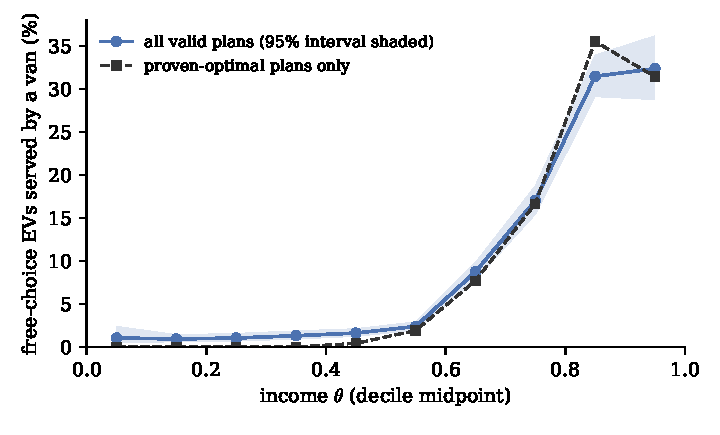
\includegraphics[width=0.66\textwidth]{figures/van_by_income.pdf}
\caption{Share of free-choice EVs served by a van, by income decile.}
\label{fig:van}
\end{figure}
\begin{table}[H]
\centering\small
\caption{Van share by income decile; 95\pct{} Wilson interval over all valid plans.}
\label{tab:deciles}
\begin{tabular}{@{}lrrrrr@{}}
\toprule
income $\theta$ & EVs & \shortstack[r]{by van\\(\%)} & \shortstack[r]{95\,\%\\interval} & \shortstack[r]{EVs\\(optimal plans)} & \shortstack[r]{by van (\%)\\(optimal plans)} \\
\midrule
0.0--0.1 & 485 & 1.0 & [0.4, 2.4] & 182 & 0.0 \\
0.1--0.2 & 2182 & 0.9 & [0.6, 1.4] & 867 & 0.0 \\
0.2--0.3 & 2050 & 1.0 & [0.7, 1.6] & 846 & 0.0 \\
0.3--0.4 & 2168 & 1.3 & [0.9, 1.9] & 692 & 0.0 \\
0.4--0.5 & 3061 & 1.6 & [1.2, 2.1] & 997 & 0.4 \\
0.5--0.6 & 3754 & 2.4 & [1.9, 2.9] & 1371 & 1.9 \\
0.6--0.7 & 2929 & 8.7 & [7.8, 9.8] & 1262 & 7.7 \\
0.7--0.8 & 1941 & 17.0 & [15.4, 18.7] & 811 & 16.6 \\
0.8--0.9 & 1408 & 31.5 & [29.1, 33.9] & 566 & 35.5 \\
0.9--1.0 & 606 & 32.3 & [28.7, 36.2] & 226 & 31.4 \\
\bottomrule
\end{tabular}

\end{table}
\begin{itemize}
  \item Overall \VanAll\pct{} of free-choice EVs get a van; van users have a mean income of \ThetaVan, station users \ThetaFCS.
  \item In optimal plans: \VanLowOpt\pct{} below $\theta=0.4$, then \VanSixSeven\pct, \VanSevenEight\pct{} and \VanEightNine\pct. The share flattens at the top (\VanNineTen\pct{} for 0.9--1.0) because the van seats run out (Section~\ref{sec:vans}).
  \item The \LowVanTL{} low-income ($\theta<0.4$) van users all come from time-limit plans (\LowVanOpt{} in optimal plans); they wait \VanWaitBot{} min on average for the van against \VanWaitTop{} min in the richest band. They are artefacts of unfinished optimisation, not a property of the model.
\end{itemize}

\subsubsection{Logistic regression}
\begin{table}[H]
\centering\small
\caption{Logistic regression of $P(\text{served by a van})$ over the \LogitN{} free-choice EVs.}
\label{tab:logit}
\begin{tabular}{@{}lrrrr@{}}
\toprule
term & coefficient & std.\ error & $z$ & $p$-value \\
\midrule
intercept & -9.036 & 0.256 & -35.2 & $<0.001$ \\
income $\theta$ & 9.806 & 0.289 & 33.9 & $<0.001$ \\
medium pressure & -0.851 & 0.085 & -10.0 & $<0.001$ \\
high pressure & 3.839 & 0.275 & 14.0 & $<0.001$ \\
$\theta\times$ high pressure & -5.715 & 0.381 & -15.0 & $<0.001$ \\
long horizon (type 2) & -0.030 & 0.066 & -0.5 & 0.649 \\
energy $E_i$ (per 10 kWh) & -0.250 & 0.056 & -4.5 & $<0.001$ \\
nearest reachable FCS (km) & 0.449 & 0.038 & 11.8 & $<0.001$ \\
\bottomrule
\end{tabular}

\end{table}
Income has a strong positive effect: $+0.1$ in $\theta$ raises the probability of a van by \AME{} percentage points on average (\AMENotHigh{} at low or medium pressure, \AMEHigh{} at high pressure). Distance to the nearest station raises it and energy demand lowers it, as the threshold formula predicts; the horizon has no effect of its own once demand pressure is included. The model classifies \LogitAcc\pct{} of EVs correctly.

\inshort{Income is the main driver of who gets a van, with a step near $\theta^{*}$; distance helps, energy hurts slightly, congestion weakens the income effect. Low-income van users exist only in unfinished plans.}

%---------------------------------------------------------------------
\subsection{Queues, priority and driving}
\label{sec:queues}
\begin{figure}[H]
\centering
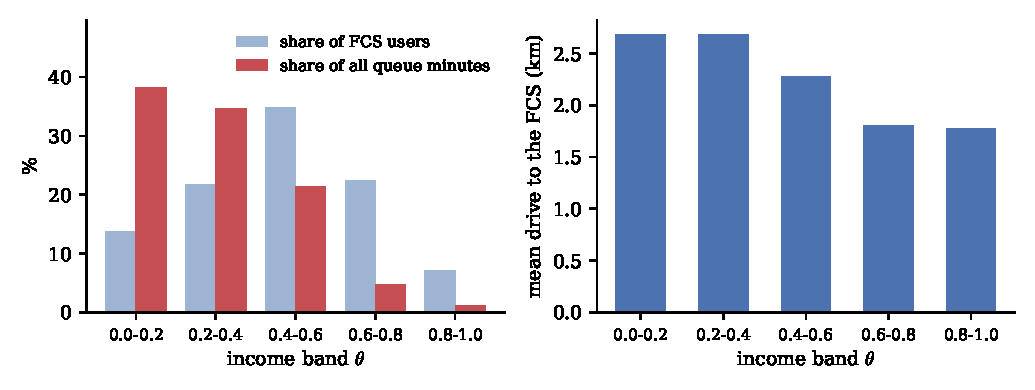
\includegraphics[width=\textwidth]{figures/queues_drive.pdf}
\caption{Left: share of station users and of all queue minutes by income band. Right: mean distance driven to the station.}
\label{fig:queues}
\end{figure}
\begin{table}[H]
\centering\footnotesize
\caption{Station users by income band.}
\label{tab:queues}
\begin{tabular}{@{}lrrrrrrrr@{}}
\toprule
income $\theta$ & \shortstack[r]{FCS\\users} & \shortstack[r]{share of\\users (\%)} & \shortstack[r]{share of queue\\minutes (\%)} & \shortstack[r]{queueing\\(\%)} & \shortstack[r]{mean queue\\(min)} & \shortstack[r]{longest\\queue (min)} & \shortstack[r]{largest\\$W_i$ (min)} & \shortstack[r]{drive to\\FCS (km)} \\
\midrule
0.0--0.2 & 2642 & 13.8 & 38.2 & 13.6 & 3.79 & 55.8 & 59.3 & 2.69 \\
0.2--0.4 & 4169 & 21.8 & 34.6 & 10.9 & 2.18 & 48.8 & 50.7 & 2.69 \\
0.4--0.6 & 6677 & 34.9 & 21.3 & 6.5 & 0.84 & 40.3 & 42.0 & 2.27 \\
0.6--0.8 & 4284 & 22.4 & 4.7 & 2.9 & 0.29 & 30.8 & 33.0 & 1.80 \\
0.8--1.0 & 1375 & 7.2 & 1.1 & 3.1 & 0.22 & 20.8 & 23.9 & 1.78 \\
\bottomrule
\end{tabular}

\end{table}
\begin{itemize}
  \item The poorest 40\pct{} are \UShareBottom\pct{} of station users but do \QShareBottom\pct{} of all queueing; the richest 20\pct{} are \UShareTop\pct{} of users and do \QShareTop\pct.
  \item Mechanism: when two EVs want the same gun, the one with the higher queueing rate $c^{\mathrm Q}(\theta)$ goes first; the gun-minute shadow prices of Section~\ref{sec:duals} show the same pattern from the dual side.
  \item Nobody queues up to their limit $W_i$; the queues follow from the cost weights alone.
  \item Low-income users drive farther (\DriveBot{} against \DriveTop{} km), although they feel the driving cost most: the free guns at the nearest stations go to customers whose time is worth more.
\end{itemize}

\inshort{Queue priority and the nearest free guns go to higher incomes; low-income customers wait and drive more. This is the cost-minimising plan under income-dependent values of time, and an equity issue an operator would have to decide on.}

%---------------------------------------------------------------------
\subsection{Peak and off-peak: demand pressure}
\label{sec:pressure}
\begin{figure}[H]
\centering
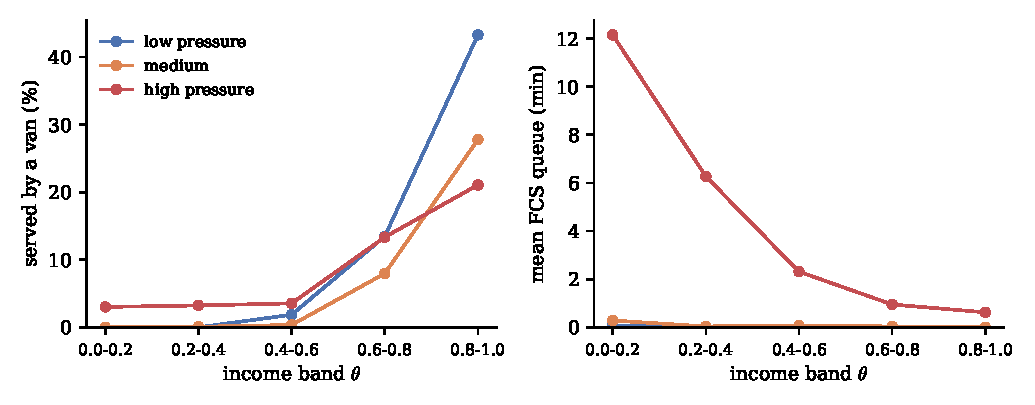
\includegraphics[width=\textwidth]{figures/pressure.pdf}
\caption{Van share and mean station queue by income band for low, medium and high demand pressure.}
\label{fig:pressure}
\end{figure}
\begin{table}[H]
\centering\footnotesize
\caption{Free-choice EVs by demand pressure.}
\label{tab:pressure}
\begin{tabular}{@{}lrrrrrrrrr@{}}
\toprule
\shortstack[l]{demand\\pressure} & EVs & \shortstack[r]{queueing\\(\%)} & \shortstack[r]{mean queue\\(min)} & \shortstack[r]{by van\\(\%)} & \shortstack[r]{by van\\$\theta$ 0.0--0.2} & \shortstack[r]{by van\\$\theta$ 0.2--0.4} & \shortstack[r]{by van\\$\theta$ 0.4--0.6} & \shortstack[r]{by van\\$\theta$ 0.6--0.8} & \shortstack[r]{by van\\$\theta$ 0.8--1.0} \\
\midrule
low & 8168 & 0.4 & 0.03 & 8.3 & 0.0 & 0.0 & 1.9 & 13.5 & 43.3 \\
medium & 5663 & 1.3 & 0.08 & 5.0 & 0.0 & 0.1 & 0.4 & 8.0 & 27.8 \\
high & 6753 & 20.9 & 4.08 & 7.0 & 3.0 & 3.2 & 3.5 & 13.4 & 21.1 \\
\bottomrule
\end{tabular}

\end{table}
\begin{itemize}
  \item Queues exist only at high pressure: \QLow, \QMid{} and \QHigh{} min on average at low, medium and high pressure; \QueuingHigh\pct{} of station users queue at high pressure.
  \item At high pressure fewer of the richest get a van (\TopLow\pct{} at low, \TopMid\pct{} at medium, \TopHigh\pct{} at high pressure): the vans are already committed.
  \item Instead, income buys priority at the station: at high pressure the richest band queues \TopQHigh{} min, the poorest 40\pct{} \LowQHigh{} min.
\end{itemize}

\inshort{Peak demand creates the queues; at peak, income buys a place at the station rather than a van.}

%---------------------------------------------------------------------
\subsection{Planning horizon and layout}
\label{sec:horizon}
\begin{figure}[H]
\centering
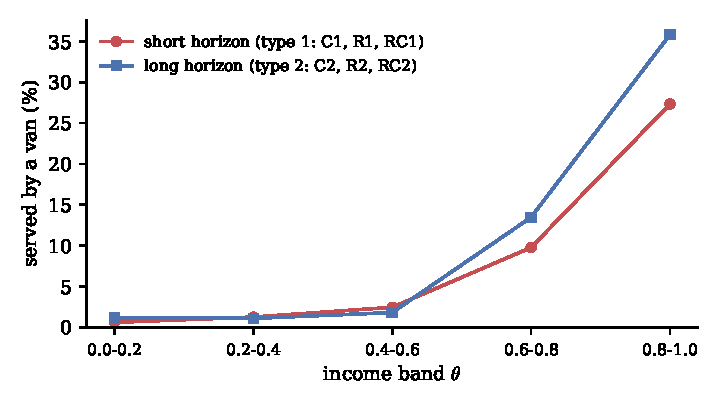
\includegraphics[width=0.66\textwidth]{figures/horizon.pdf}
\caption{Van share by income band, short-horizon against long-horizon families.}
\label{fig:horizon}
\end{figure}
\begin{table}[H]
\centering\footnotesize
\caption{Van share by family and income band.}
\label{tab:families}
\begin{tabular}{@{}llrrrrrrrr@{}}
\toprule
family & horizon & EVs & \shortstack[r]{mean\\pressure} & \shortstack[r]{by van\\(\%)} & \shortstack[r]{by van\\$\theta$ 0.0--0.2} & \shortstack[r]{by van\\$\theta$ 0.2--0.4} & \shortstack[r]{by van\\$\theta$ 0.4--0.6} & \shortstack[r]{by van\\$\theta$ 0.6--0.8} & \shortstack[r]{by van\\$\theta$ 0.8--1.0} \\
\midrule
C1 & short & 4104 & 0.38 & 6.9 & 0.9 & 1.5 & 0.4 & 6.2 & 37.0 \\
C2 & long & 3771 & 0.29 & 8.9 & 1.4 & 0.8 & 3.9 & 13.5 & 36.8 \\
R1 & short & 2493 & 0.69 & 5.6 & 0.3 & 0.7 & 2.5 & 13.7 & 17.5 \\
R2 & long & 5082 & 0.56 & 5.9 & 1.5 & 1.4 & 1.0 & 11.2 & 49.2 \\
RC1 & short & 1454 & 0.69 & 7.8 & 0.4 & 1.8 & 6.5 & 20.1 & 16.2 \\
RC2 & long & 3680 & 0.46 & 7.2 & 0.6 & 0.9 & 1.4 & 17.4 & 27.2 \\
\bottomrule
\end{tabular}

\end{table}
High-income customers get a van more often with a long horizon (\TopLong\pct{} against \TopShort\pct{} in the top band), most clearly for R and RC; for the clustered layout C the two horizons are close. Short horizons also mean higher demand pressure (\PressShort{} against \PressLong); with pressure in the regression the horizon has no separate effect.

\inshort{The horizon matters through congestion and through the vans' time budget (next section).}

%---------------------------------------------------------------------
\subsection{The vans: what limits them}
\label{sec:vans}
\begin{table}[H]
\centering\small
\caption{Use of the \VansN{} vans dispatched in the valid plans.}
\label{tab:vans}
\begin{tabular}{@{}lrrl@{}}
\toprule
measure & mean & median & at the limit \\
\midrule
vans dispatched (all valid plans) & 1039 &  &  \\
stops per van & 4.91 & 6 & 54.5\,\% at $Q_m=6$ \\
battery drawn (kWh) & 110.4 & 117.9 & 28.4\,\% above 90\,\% of $B_m$ \\
back at depot ($\%$ of $T$) & 73.0 & 75.3 & 20.4\,\% after 90\,\% of $T$ \\
van km & 32.8 & 30.6 &  \\
\bottomrule
\end{tabular}

\end{table}
\begin{table}[H]
\centering\small
\caption{Which van resource is closest to its limit (largest share used of seats, battery and time).}
\label{tab:vanstight}
\begin{tabular}{@{}lrr@{}}
\toprule
tightest van resource & vans & share (\%) \\
\midrule
seats ($Q_m=6$) & 636 & 61.2 \\
battery ($B_m=150$ kWh) & 88 & 8.5 \\
time ($T$) & 315 & 30.3 \\
\bottomrule
\end{tabular}

\end{table}
\begin{table}[H]
\centering\small
\caption{Van use by family.}
\label{tab:vansfamily}
\begin{tabular}{@{}lrrrrr@{}}
\toprule
family & vans & \shortstack[r]{stops\\per van} & \shortstack[r]{back at depot\\(\% of $T$)} & \shortstack[r]{tightest:\\seats (\%)} & \shortstack[r]{tightest:\\time (\%)} \\
\midrule
C1 & 193 & 5.84 & 67.3 & 99.0 & 0.5 \\
C2 & 153 & 5.64 & 67.3 & 68.6 & 2.6 \\
R1 & 181 & 3.24 & 91.3 & 0.0 & 100.0 \\
R2 & 222 & 5.72 & 63.6 & 97.7 & 2.3 \\
RC1 & 105 & 2.57 & 88.5 & 0.0 & 100.0 \\
RC2 & 185 & 5.32 & 67.9 & 66.5 & 10.3 \\
\bottomrule
\end{tabular}

\end{table}
\begin{figure}[H]
\centering
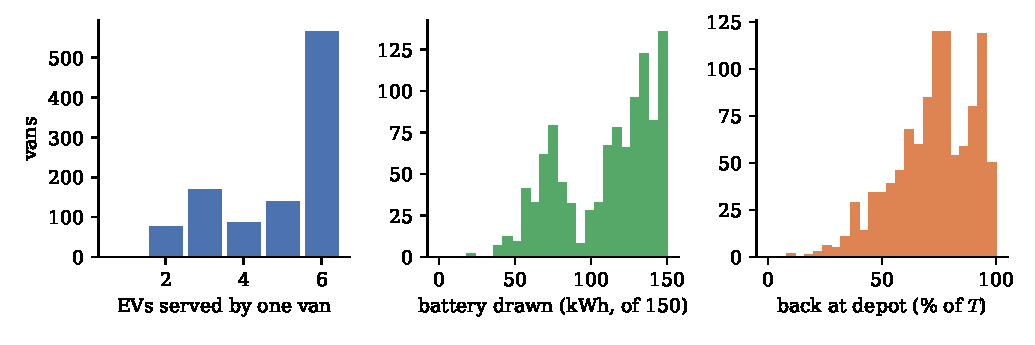
\includegraphics[width=\textwidth]{figures/c_vans.pdf}
\caption{EVs per van, battery drawn and return time of every dispatched van.}
\label{fig:vans}
\end{figure}
\begin{itemize}
  \item \VansFull\pct{} of vans are full (6 EVs). \VanSeatsStranded\pct{} of all van seats are taken by stranded EVs; the rest go to free-choice customers, mostly rich.
  \item Seats are the tightest resource for \TightSeats\pct{} of vans, time for \TightTime\pct{} and the battery for only \TightBatt\pct.
  \item The split follows the horizon: in C1, C2, R2 and RC2 (long or clustered) vans fill their 6 seats; in R1 and RC1 (230--240 minutes) every van runs out of time with only 2.6--3.2 EVs served.
\end{itemize}

\inshort{Vans are filled first by stranded EVs. With a long horizon a van's limit is its 6 seats; with a short one, its time. The battery is rarely the limit.}

%---------------------------------------------------------------------
\subsection{Money paid and perceived cost: equity}
\label{sec:equity}
\begin{figure}[H]
\centering
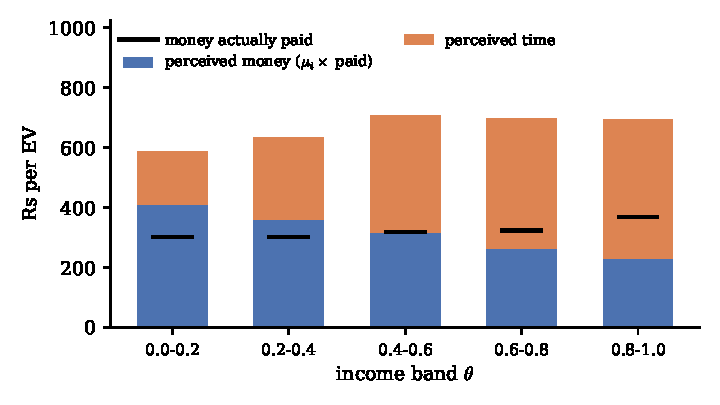
\includegraphics[width=0.66\textwidth]{figures/costs.pdf}
\caption{Money paid and perceived cost per EV by income band.}
\label{fig:costs}
\end{figure}
\begin{table}[H]
\centering\footnotesize
\caption{Shares of money paid and perceived cost by income band.}
\label{tab:equity}
\begin{tabular}{@{}lrrrrrr@{}}
\toprule
income $\theta$ & \shortstack[r]{share of\\EVs (\%)} & \shortstack[r]{share of\\money paid (\%)} & \shortstack[r]{share of\\perceived cost (\%)} & \shortstack[r]{perceived per\\Rs paid} & \shortstack[r]{time share of\\perceived (\%)} & \shortstack[r]{paid per\\kWh (Rs)} \\
\midrule
0.0--0.2 & 13.0 & 12.3 & 11.3 & 1.94 & 29.9 & 15.7 \\
0.2--0.4 & 20.5 & 19.3 & 19.3 & 2.10 & 43.2 & 15.7 \\
0.4--0.6 & 33.1 & 33.1 & 34.8 & 2.22 & 55.3 & 15.7 \\
0.6--0.8 & 23.7 & 24.0 & 24.5 & 2.15 & 62.1 & 16.5 \\
0.8--1.0 & 9.8 & 11.3 & 10.1 & 1.88 & 66.9 & 18.4 \\
\bottomrule
\end{tabular}

\end{table}
\begin{itemize}
  \item Perceived cost per rupee paid is similar at both ends (\PerRsBot{} for the poorest band, \PerRsTop{} for the richest) and highest in the middle: the poor feel money strongly, the rich feel time strongly.
  \item The composition differs: time is \TimeShareBot\pct{} of the perceived cost of the poorest and \TimeShareTop\pct{} of the richest.
  \item The rich pay more per kWh (\PerKWhTop{} against \PerKWhBot{} Rs) because more of them use the van; the poor pay less but wait and drive more (Section~\ref{sec:queues}).
\end{itemize}

\inshort{Each group bears the cost it minds least in rupee terms: the poor wait and drive, the rich pay. Perceived cost per rupee is similar at the two ends of the income range.}

%---------------------------------------------------------------------
\subsection{Instance size and computation}
\label{sec:computation}
\begin{table}[H]
\centering\footnotesize
\caption{Model size and solver behaviour by instance size.}
\label{tab:model}
\begin{tabular}{@{}rrrrrrrr@{}}
\toprule
$n$ & \shortstack[r]{binary\\variables} & \shortstack[r]{continuous\\variables} & constraints & \shortstack[r]{build\\time (s)} & \shortstack[r]{median\\B\&B nodes} & \shortstack[r]{median gain over\\greedy (\%)} & \shortstack[r]{greedy plan\\found (\%)} \\
\midrule
10 & 812 & 30 & 1,917 & 0.0 & 1 & 0.5 & 98.2 \\
20 & 2,669 & 60 & 6,948 & 0.2 & 1 & 0.7 & 98.2 \\
30 & 5,641 & 90 & 16,316 & 0.4 & 132 & 0.7 & 98.2 \\
40 & 9,659 & 120 & 28,449 & 0.8 & 2,664 & 2.5 & 96.4 \\
50 & 14,696 & 150 & 42,512 & 1.2 & 1,499 & 4.0 & 92.9 \\
60 & 20,880 & 180 & 62,074 & 1.9 & 1,202 & 4.9 & 87.5 \\
70 & 28,147 & 210 & 86,115 & 2.3 & 1,128 & 5.1 & 78.6 \\
80 & 36,428 & 240 & 111,083 & 2.9 & 588 & 4.3 & 69.6 \\
90 & 45,834 & 270 & 139,872 & 4.5 & 1 & 4.9 & 66.1 \\
100 & 56,222 & 300 & 171,924 & 4.2 & 275 & 4.5 & 60.7 \\
\bottomrule
\end{tabular}

\end{table}
The model grows quickly: about \BinHundred{} binary variables and \ConHundred{} constraints at $n=100$, mostly the van arcs $x_{ijm}$ and the pairwise gun-order constraints. The greedy start plan exists for 98\pct{} of small instances but only 61\pct{} at $n=100$ (it fails once the queue limits $W_i$ apply); Gurobi improves on it by about 4--5\pct{} for larger instances. The greedy plan used the cost rule in \GreedyCost{} instances, the earliest-finish rule in \GreedyFinish, and none was found in \GreedyNone.

\inshort{Problem size grows roughly with $n^2$; beyond $n\approx40$ the 300\,s limit binds, and the greedy start often fails for large congested instances.}

%---------------------------------------------------------------------
\subsection{Infeasible and unsolved instances}
\label{sec:infeasible}
\begin{table}[H]
\centering\small
\caption{Infeasible instances (Gurobi's verdict).}
\label{tab:infeasible}
\begin{tabular}{@{}lrrr@{}}
\toprule
family & infeasible instances & smallest $n$ & largest $n$ \\
\midrule
R1 & 29 & 50 & 100 \\
RC1 & 22 & 10 & 100 \\
\bottomrule
\end{tabular}

\end{table}
\begin{itemize}
  \item All \InfTotal{} infeasible instances are in the short-horizon families R1 and RC1, and in all \InfProven{} of them the data alone already prove it: some EV cannot be charged by $T$ even with a free gun or a van straight away. Example: \LateExample. Income plays no role.
  \item The \NNone{} unsolved instances are the most congested ones: their mean demand pressure is \UnsolvedPress, against \SolvedPressSame{} for solved instances of the same family and size. They need a longer time limit or a better start plan.
\end{itemize}

\inshort{Infeasibility comes from late requests in the short-horizon families, not from the income model; the unsolved instances are the most congested.}

%---------------------------------------------------------------------
\subsection{Sensitivity to the income distribution}
\label{sec:beta}
The run used Beta(2,2). If the probability of a van at each income level stayed as observed, other income distributions would give the van shares below (a reweighting of the decile shares; the plans themselves would adapt, so this is a first-order estimate).
\begin{table}[H]
\centering\small
\caption{Expected van share of free-choice EVs under other income distributions.}
\label{tab:beta}
\begin{tabular}{@{}lrrr@{}}
\toprule
income distribution & mean $\theta$ & EVs with $\theta\ge0.6$ (\%) & expected van share (\%) \\
\midrule
Beta(1,1) uniform & 0.50 & 40.0 & 9.8 \\
Beta(2,2) (used) & 0.50 & 35.2 & 7.4 \\
Beta(2,5) mostly low income & 0.29 & 4.1 & 1.6 \\
Beta(5,2) mostly high income & 0.71 & 76.7 & 17.0 \\
Beta(0.5,0.5) polarised & 0.50 & 43.8 & 12.1 \\
\bottomrule
\end{tabular}

\end{table}
A population leaning to high incomes (Beta(5,2)) would roughly double the van share; one leaning to low incomes (Beta(2,5)) would almost remove vans for free-choice customers. Because vans are capacity-limited, the high-income case would also push more rich customers to stations, so the true shares would be lower than this estimate at the top.

\inshort{Who uses vans depends strongly on the income mix; calibrating $\theta$ to real EV-owner incomes matters (Section~\ref{sec:calibration}).}

%---------------------------------------------------------------------
\subsection{Robustness and caveats}
\label{sec:robust}
\begin{itemize}
  \item \textbf{Placeholder parameters.} Directions come from the formulation, sizes from the placeholder values; the tornado table shows which ones matter.
  \item \textbf{Time-limit plans.} Valid but not proven optimal; they contain artefacts such as low-income van users with long waits. Results that matter are checked on optimal plans.
  \item \textbf{Unsolved instances.} The most congested R1 and RC1 instances are missing, so the analysis under-represents extreme congestion.
  \item \textbf{Shadow prices are conditional} on the plan's decisions; values of discrete resources need re-solving.
  \item \textbf{Demand pressure is a proxy}: it ignores travel time and counts a van as one charger.
  \item \textbf{Income is independent of location}: richer and poorer neighbourhoods are not modelled.
\end{itemize}

%---------------------------------------------------------------------
\subsection{Calibration and extensions}
\label{sec:calibration}
Indian sources that could replace the placeholders:
\begin{itemize}
  \item \textbf{Income of car owners.} Car ownership by income quintile from the 2022--23 household consumption survey (\href{https://www.dataforindia.com/vehicle-ownership/}{Data for India}): under 5\pct{} in the bottom four rural quintiles, about 30\pct{} in the top urban quintile. With $\theta$ read as an income percentile this gives a distribution strongly skewed to high incomes, unlike Beta(2,2).
  \item \textbf{Use segments.} Vahan registrations split transport (taxi, commercial) and non-transport (private) vehicles (\href{https://dataful.in/datasets/21146/}{Dataful}); CSTEP surveyed 878 personal and 855 commercial EV users in four cities (\href{https://cstep.in/?p=1521}{CSTEP}). A taxi's value of time is the driver's lost earnings, not household income: a second attribute ``segment'' would capture it.
  \item \textbf{Value of time.} About Rs 609 per hour for Bengaluru commuters (\href{https://www.nber.org/papers/w25218.pdf}{NBER study}); with our lines that corresponds to $c^{\mathrm D}\approx10$\,Rs/min, i.e.\ $\theta\approx0.6$.
  \item \textbf{Extensions.} Re-solve with $\pm$ parameters to obtain the discrete shadow prices (value of one more van, gun or seat); add charging segments; correlate income with location.
\end{itemize}

%=====================================================================
\section{Summary of findings}
\begin{enumerate}
  \item The run is sound: \NValid{} valid plans, infeasibility caused by the data.
  \item Income decides who gets a van, with a threshold near $\theta^{*}=\ThetaStar$ predicted by the formulation and confirmed by the optimal plans.
  \item Vans leave for stranded EVs; their spare seats go to the rich. Seats limit vans in long horizons, time in short ones.
  \item Low-income customers absorb queues and drive farther; at peak demand income buys queue priority rather than a van.
  \item Shadow prices: gun-minutes cost \GunMean{} Rs when scarce, paid by poorer customers waiting behind richer ones; patience limits and the deadline have zero marginal value for fixed plans; one more kW of station power is worth about \DPFmean{} Rs per instance.
  \item The objective is most sensitive to the station tariff, the money sensitivity of low incomes, the value of charging time of high incomes and the grid price; the threshold is most sensitive to the value of charging time of high incomes, the van energy price and the van tariff.
  \item The income distribution changes the van share strongly; calibrating it to Indian data is the most important next step.
\end{enumerate}

\vspace{6pt}
{\footnotesize Generated from \texttt{../results.csv}, \texttt{../analysis/ev\_level.csv} and the plans by \texttt{make\_figures.py}, \texttt{compute\_duals.py} and \texttt{make\_comprehensive.py} in this folder.}

\end{document}
